\documentclass[twocolumn,final]{svjour3}

\newcommand{\thetitle}{Linear Representation of Network Traffic}
\newcommand{\theauthors}{
  Stefan~Karpinski \and
  Elizabeth~M.~Belding \and
  Kevin~C.~Almeroth \and
  John~R.~Gilbert
}

%\usepackage{type1cm}
%\usepackage[pdftex]{graphicx}
\usepackage[labelfont=bf,small]{caption}
\usepackage[font=small,labelfont=bf,position=top,nearskip=0em]{subfig}
\usepackage{cite,amsmath,amssymb,rotating,multirow,bigstrut,url,wrapfig,relsize,paralist,array}
\usepackage[hyperfigures,bookmarks,bookmarksopen,bookmarksnumbered,colorlinks,linkcolor=black,citecolor=black,filecolor=blue,menucolor=black,pagecolor=blue,frenchlinks=true,pdftitle={\thetitle}]{hyperref}
\usepackage{mathtools}

\title{\thetitle}
\author{\theauthors}
\institute{
  S.~Karpinski \and
  E.~Belding \and
  K.~Almeroth \and
  J.~Gilbert \\
  Department of Computer Science \\
  University of California, Santa Barbara (USA) \\
  Email: \texttt{\{sgk,ebelding,almeroth,gilbert\}@cs.ucsb.edu}
}

%!TEX root = /Users/stefan/projects/papers/paper.4/paper.tex

%% LABELING COMMANDS
\renewcommand{\sec}[1]{\label{sec:#1}}
\newcommand{\eqn}[1]{\label{eqn:#1}}
\newcommand{\fig}[1]{\label{fig:#1}}
\newcommand{\tab}[1]{\label{tab:#1}}
\newcommand{\thm}[1]{\label{thm:#1}}
\newcommand{\defn}[1]{\label{def:#1}}

%% REFERENCING COMMANDS
\newcommand{\Appendix}[1]{\hyperref[sec:#1]{Appendix~\ref*{sec:#1}}}
\newcommand{\Section}[1]{\hyperref[sec:#1]{Section~\ref*{sec:#1}}}
\newcommand{\Equation}[1]{\hyperref[eqn:#1]{Equation~\ref*{eqn:#1}}}
\newcommand{\Figure}[1]{\hyperref[fig:#1]{Figure~\ref*{fig:#1}}}
\newcommand{\Table}[1]{\hyperref[tab:#1]{Table~\ref*{tab:#1}}}
\newcommand{\Theorem}[1]{\hyperref[thm:#1]{Theorem~\ref*{thm:#1}}}
\newcommand{\Definition}[1]{\hyperref[def:#1]{Definition~\ref*{def:#1}}}

%% MATHEMATICAL NOTATIONS

% common algebraic domains
\newcommand{\N}{\mathbb{N}}
\newcommand{\Z}{\mathbb{Z}}
\newcommand{\Q}{\mathbb{Q}}
\newcommand{\R}{\mathbb{R}}

% standard operators & functors
\renewcommand{\Pr}{\mathrm{Pr}}
\newcommand{\Image}{\text{Im}}
\newcommand{\Kernel}{\text{Ker}}

% common constructs
\newcommand{\abs}[1]{{\left|#1\right|}}
\newcommand{\absx}[1]{{|#1|}}
\newcommand{\card}[1]{{\left|#1\right|}}
\newcommand{\cardx}[1]{{|#1|}}
\newcommand{\norm}[1]{{\lVert#1\rVert}}
\newcommand{\normx}[1]{{\Vert#1\Vert}}
\newcommand{\set}[1]{{\left\{#1\right\}}}
\newcommand{\setx}[1]{{\{#1\}}}
\newcommand{\parens}[1]{{\left(#1\right)}}
\newcommand{\parensx}[1]{{(#1)}}
\newcommand{\bracket}[1]{{\left[#1\right]}}
\newcommand{\bracketx}[1]{{[#1]}}
\newcommand{\seq}[1]{{\left<#1\right>}}
\newcommand{\seqx}[1]{{\lvert#1\rvert}}
\newcommand{\tuple}[1]{{\left<#1\right>}}
\newcommand{\tuplex}[1]{{\lvert#1\rvert}}
\newcommand{\floor}[1]{{\left\lfloor#1\right\rfloor}}
\newcommand{\floorx}[1]{{\lfloor#1\rfloor}}
\newcommand{\ceil}[1]{{\left\lceil#1\right\rceil}}
\newcommand{\ceilx}[1]{{\lceil#1\rceil}}
\newcommand{\round}[1]{{\left[#1\right]}}
\newcommand{\roundx}[1]{{[#1]}}
\newcommand{\fracx}[2]{{#1/#2}}
\newcommand{\fracp}[2]{{\left(\frac{#1}{#2}\right)}}
\newcommand{\fracpx}[2]{{(#1/#2)}}

% standard notations
\newcommand{\trans}[1]{{#1}^T}
\newcommand{\inner}[2]{{#1}\cdot{#2}}
\newcommand{\cross}{\times}
\newcommand{\tensor}{\otimes}
\newcommand{\directsum}{\oplus}
\newcommand{\iso}{\cong}
\newcommand{\union}{\cup}
\newcommand{\inter}{\cap}
\newcommand{\Union}{\bigcup}
\newcommand{\Inter}{\bigcap}
\newcommand{\conj}{\wedge}
\newcommand{\disj}{\vee}
\newcommand{\Conj}{\bigwedge}
\newcommand{\Disj}{\bigvee}
\newcommand{\defeq}{=}
\renewcommand{\emptyset}{\varnothing}
\renewcommand{\setminus}{\,\raisebox{1pt}{$\smallsetminus$}\,}

% non-standard notations
\newcommand{\ones}[1]{\mathbf{1}_{#1}}
\newcommand{\zeros}[1]{\mathbf{0}_{#1}}
\newcommand{\mat}[1]{\mathbf{#1}}
\newcommand{\mean}[1]{\bar{#1}}
\newcommand{\mathsym}[1]{\text{\textsf{#1}}}
\newcommand{\e}{\vec{e}}

% special symbols and such
\newcommand{\FlowSet}[1]{\mathcal{#1}}
\newcommand{\Flows}{\FlowSet{F}}
\newcommand{\Types}{\FlowSet{Y}}
\newcommand{\Nodes}{\FlowSet{N}}
\newcommand{\Times}{\FlowSet{T}}
\newcommand{\Sizes}{\FlowSet{Z}}
\newcommand{\Ivals}{\FlowSet{V}}
\newcommand{\SizeSeq}{\Sizes^\N}
\newcommand{\IvalSeq}{\Ivals^\N}
\newcommand{\Traffic}{\Flows^*}

\newcommand{\FlowElt}[1]{\mathsym{#1}}
\newcommand{\flow}{\FlowElt{flow}}
\newcommand{\type}{\FlowElt{type}}
\newcommand{\src}{\FlowElt{src}}
\newcommand{\dst}{\FlowElt{dst}}
\newcommand{\start}{\FlowElt{start}}
\newcommand{\size}{\FlowElt{size}}
\newcommand{\ival}{\FlowElt{ival}}
\newcommand{\pkts}{\FlowElt{pkts}}
\newcommand{\sizes}{\FlowElt{sizes}}
\newcommand{\ivals}{\FlowElt{ivals}}
\renewcommand{\time}{\FlowElt{time}}

\newcommand{\Qf}{\mathcal{Q}}
\newcommand{\Qt}{\Qf_{\text{time}}}
\newcommand{\Qb}{\Qf_{\text{byte}}}
\newcommand{\Qi}{\Qf_{\text{ival}}}
\newcommand{\Di}{\Qf^{-1}_{\text{ival}}}

\newcommand{\pbd}{\mathsym{pbd}}
\newcommand{\FlowVec}{\mathcal{X}}

%% FORMATTING BEHAVIORS
\newcommand{\caps}[1]{{\smaller{#1}}}
\newcommand{\latin}[1]{\textit{#1}}
\newcommand{\defterm}[1]{\textit{#1}}
\newcommand{\newfootnote}[2]{\newcommand{#1}{\footnote{#2} }}
\renewcommand{\bullet}{\raisebox{2pt}{$\centerdot$}}

%% MISCELLANEOUS COMMANDS
\newcommand{\FHC}{Hern\'andez-Campos~\textit{et~al.}}
\newcommand{\class}[1]{\textsc{#1}}
\newcommand{\model}[1]{\textsf{#1}}
\newcommand{\RFC}[1]{\caps{RFC}~{#1}}
\newcommand{\tmix}{T\caps{MIX}}


\graphicspath{{graphics/}}

\begin{document}
\maketitle

\begin{abstract}
We propose a representation of wireless workload patterns as large, sparse matrices and provide a method for stochastically generating experimental workload from a given matrix. The essential property of the algebraic representation is that the summation of vectors naturally yields a faithful description of the aggregate behavior of the corresponding flows. This deceptively simple property allows us to express many common concepts from traffic modeling succinctly in terms of a few linear transformations. The algebraic representation has many benefits: 1)~it makes the meaning of generally understood but vague concepts, such as ``uniform behavior,'' mathematically precise and unambiguous; 2)~it allows us to see clearly, through the lens of linear algebra, the implications of common modeling assumptions; 3)~the implementation of traffic models becomes unprecedentedly simple and orthogonal, requiring only a handful of high-level matrix operations, which can be freely composed; 4)~the vast body of algebraic theory and highly optimized numerical linear software may immediately be applied to traffic modeling. We use the paired differential simulation methodology introduced by the authors in previous work to experimentally demonstrate that the general matrix model accurately reproduces realistic network performance~\cite{Karpinski07:realism,Karpinski07:cbr-failure}. We use the same experimental methodology to explore the implications of various assumptions and simplifications that are commonly made in traffic modeling.
%We demonstrate experimentally that the general matrix model accurately reproduces network performance metrics, using the differential simulation methodology introduced in~\cite{Karpinski07:realism} and applied in~\cite{Karpinski07:cbr-failure} to common uniform traffic models. A range of common modeling approaches are implemented in the general matrix model and evaluated experimentally.
%
%We demonstrate how linear algebra can be effectively used to represent and perform computations with traffic behaviors in wireless networks. Moreover, we map common concepts and techniques from traffic modeling into this new algebraic domain, showing how they can be expressed with mathematical precision and succinctness, while simultaneously being made clearer and more general. We demonstrate experimentally that the general matrix model accurately reproduces network performance metrics, using the differential simulation methodology introduced in~\cite{Karpinski07:realism} and applied in~\cite{Karpinski07:cbr-failure} to discredit the common constant bit-rate model. A range of common modeling approaches are implemented in the general matrix model and evaluated experimentally. We conclude with future directions for modeling research based on the new algebraic framework.
\end{abstract}

% The model of flow behavior implicit in non-negative matrix factoriation technique is that flow behavior is a composite of some limited set of basic behaviors---and that fractions of each flow ``belong'' to each behavior. This is not an \latin{a priori} unreasonable hypothesis. Contrast that with the assumptions underlying uniform and marginal simplifications of traffic behavior, which can be seen to be intuitively unreasonable without ever conducting and actual experiment or calculation.

\keywords{
  traffic modeling \and
  traffic analysis \and
  workload generation \and
  wireless networks \and
  wireless simulation \and
  linear algebra \and
  non-negative matrix factorization
}

\section{Introduction}\label{sec:intro}

\newfootnote{\flownote}{We use the common definition of a \textit{flow} as a sequence of packets sharing the same  ``5-tuple'': \caps{IP} protocol type, source and destination nodes, and \caps{TCP/UDP} port numbers.}

\newfootnote{\marginalnote}{The statistical term ``marginal'' refers to the margins of actuarial tables formerly used for statistical computations. The rows and columns of the table represent possible values of two properties. Each entry in a table contains a count of the number of events falling into the joint category for that row and column. The margins contain sums of the rows and columns, thus giving the unconditional distributions of each property.}

More than twenty years of research in analysis and modeling of network traffic have yielded tremendous advances in our understanding of the complex behaviors that emerge from the interaction of millions of humans and computers on the Internet and in local-area networks (\caps{LAN}s).
Both traffic analysis and realistic workload generation, however, remain active areas of research with many unanswered questions.
One of the major challenges of modeling whole-network traffic is the interdependence of packet, flow\flownote and node behaviors.
Three types of simplifying assumptions are commonly applied in both analysis and generation:
\begin{enumerate}
\item \textbf{Uniform:} that traffic properties are uniformly distributed. For example, assuming that  all nodes in a network have equal probability of being the source or destination of each flow.
Another common example is the assumption that all packet sizes and inter-packet intervals are the same; this is commonly known as the ``constant bit-rate'' (\caps{CBR}) model.
\item \textbf{Marginal:} that traffic properties share a single, common \emph{marginal}\marginalnote distribution across the entire network, and individual values are drawn independently and unconditionally from this shared distribution.
For example, assuming that a single distribution of packet sizes describes all flows in a network, as compared to equipping each flow with its own specific distribution of sizes.
\item \textbf{Conditional:} that traffic behaves marginally within equivalence classes defined by certain conditions.
The assumption, for example, that all flows emanating from a common source node share the same packet size distribution is a conditional model, conditioned on the source nodes.
\end{enumerate}
We would be arguing against a straw man if we implied that researchers who apply these assumptions actually believe them to be true.
They clearly are not:
different nodes initiate and receive drastically different numbers of packets and flows;
flows have drastically different packet size distributions.
Simply considering intuitive examples of common behavior illustrates this amply:
BitTorrent users \latin{vs.} occasional email checkers;
downloading a large file \latin{vs.} typing in an \caps{SSH} session.

% In short, the reason is that these assumptions drastically simplify both traffic analysis and workload generation.
% If we ignore the interdependencies that make analysis difficult, the difficulties simply evaporate. 
% This immediately begs the question of whether these assumptions are benign.
% Does assuming uniformity or marginality of network behavior distort the properties and metrics we are trying to analyze and replicate?
% This paper answers that question: we cannot stick our heads in the sand and pretend that network behaviors are uniform or marginal without severely distorting crucial network performance metrics.

% TODO: is this paragraph necessary?
% The second reason why uniformity and marginality assumptions are so commonly used is that there are no generally accepted alternatives for representing or analyzing traffic.
% The difficulty lies in the high-dimensional and stochastic nature of network behaviors.
% Suppose, for example, that we assume that packet sizes and inter-packet intervals are drawn independently from some given distribution for each flow.
% In the terminology introduced above, this is a flow-conditional packet behavior model.
% Prior research has indicated that, given accurate per-flow distributions, and keeping all other aspects of network behavior fixed, this simplification does not distort experimental performance metrics~\cite{Karpinski07:realism}.
% In this model, however, each flow must have its own specific, realistic pair of distributions for packet size and inter-packet intervals.
% Moreover, the ``distribution of distributions'' across the entire network must simultaneously be realistic.
% Modeling such distributions of distributions realistically for entire networks is currently an unsolved problem; we begin to address it here.

If no one actually believes that assumptions of uniformity and marginality accurately describe network behavior, then why are these assumptions so common?
There are two reasons.
The first is that these assumptions drastically simplify both traffic analysis and workload generation, making them tractable problems.
% If we ignore the interdependencies that make analysis difficult, the difficulties simply evaporate. 
% This immediately begs the question of whether these assumptions are benign.
% Does assuming uniformity or marginality of network behavior distort the properties and metrics we are trying to understand?
% This paper answers that question.
The second is that there are no generally accepted alternatives for representing and simplifying traffic patterns that allow effective analysis and generation without assuming uniformity or marginality.
% Representing complex multi-level network behaviors in a way that does not make these simplifying assumptions but allows effective traffic analysis and workload generation is currently an unsolved problem;
% we begin to address it here.

% This paper answers that question: we cannot stick our heads in the sand and pretend that network behaviors are uniform or marginal without severely distorting crucial network performance metrics.

Fundamentally, uniform, marginal and conditional models are applied so that network traffic behavior can be represented using a manageable collection of empirical or analytical statistical distributions.
Reduction in representation size and complexity makes analysis and generation feasible.
From this perspective, three questions immediately present themselves:
\begin{enumerate}
\item Do these assumptions distort the metrics we are trying to analyze, replicate, and predict?
\item Can we represent ``unreduced'' network behavior such that analysis and generation remain tractable?
\item Are there better ways to simplify and reduce the representation of network behavior?
\end{enumerate}
This paper answers all three questions. We begin, however by answering the second problem and  
using our solution to address the other two questions.
% transforming the unreduced representation of traffic into it's uniform, marginal or conditional counterparts.

To represent unreduced network behavior practically, we propose the concept of a \emph{linear representation} of network traffic.
A linear representation of traffic maps each flow to a vector, such that the following linearity condition is satisfied:
\begin{quote}
The sum of the representations of two flows is a vector that represents the aggregate behavior of the two flows.
\end{quote}
The complete behavior of a network is expressed as a matrix of such vectors, having one row per flow.
Linear representations express full network behavior, without imposing assumptions of uniformity or marginality, yet still allow effective traffic analysis and workload generation.
We present a specific linear representation, called the general matrix model (\caps{GMM}), and demonstrate experimentally that this model generates wireless workload that accurately reproduces the performance characteristics of real wireless network traffic.

\newfootnote{\ranknote}{For uniform and marginal assumptions, the multiplication matrix has rank 1  since all rows and columns are identical. In the conditional case, the rank of the matrix is the number of conditioning classes.}

To address the the other two questions, we begin with a simple observation.
In linear representations of traffic, uniform, marginal and conditional assumptions are assertions of equality between the rows and columns of the traffic matrix.
Moreover, real traffic matrices can be transformed into uniform, marginal and conditional forms through very simple matrix multiplications.
These transformations, however, are extremely destructive: the matrices are degenerate with very low rank, so multiplication destroys almost all information in the original traffic matrix.
We demonstrate experimentally, that this loss of information is not benign:
uniform and marginal traffic models severely distorting crucial network performance metrics.

%!TEX root = ../paper.tex

\begin{figure*}[!t]
\begin{center}
\subfloat[node: real]
{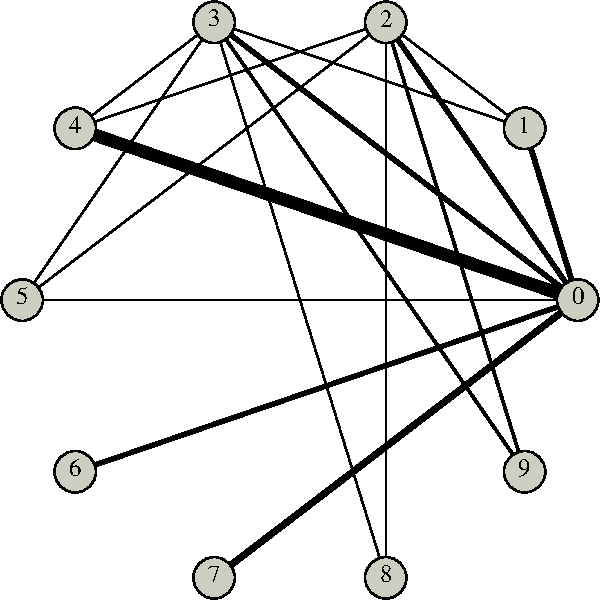
\includegraphics[width=1.335in]{flow_topology_trace}\label{fig:flow-topology-trace}}
\subfloat[node: uniform]
{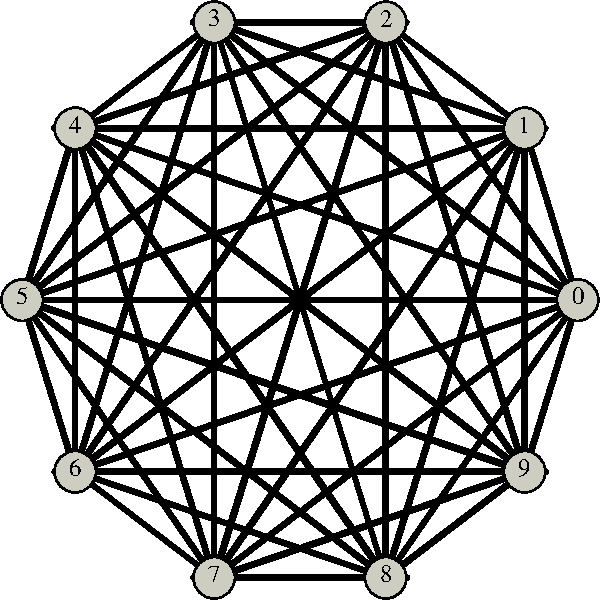
\includegraphics[width=1.335in]{flow_topology_uniform}\label{fig:flow-topology-uniform}}
\subfloat[flow: real]
{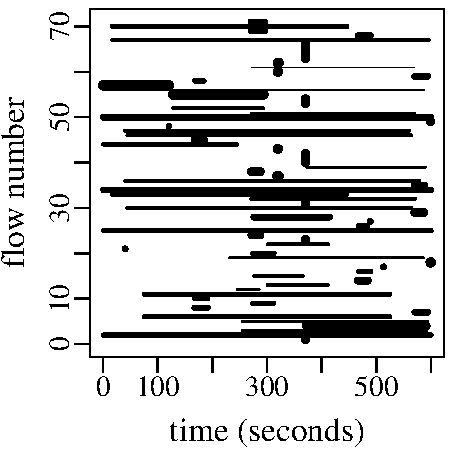
\includegraphics[width=1.335in]{flow_behavior_trace}\label{fig:flow-behavior-trace}}
\subfloat[flow: uniform]
{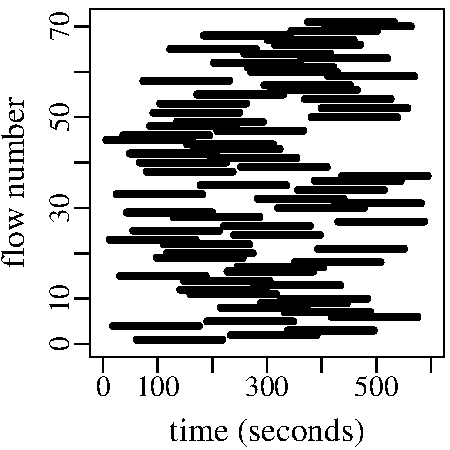
\includegraphics[width=1.335in]{flow_behavior_uniform}\label{fig:flow-behavior-uniform}}
\subfloat[packet]
{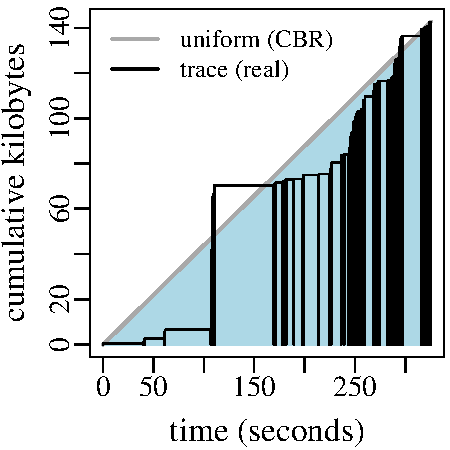
\includegraphics[width=1.335in]{flow_packet_behavior}\label{fig:packet-behavior}}
\caption{Examples illustrating real versus uniform behaviors at the node, flow and packet levels. Figures \ref{fig:flow-topology-trace} and \ref{fig:flow-topology-uniform} show example node behaviors. The width of each line is proportional to the logarithm of the number of flows between the nodes (zero is the Internet gateway). Uniform and trace flow behavior examples are plotted in Figures \ref{fig:flow-behavior-trace} and \ref{fig:flow-behavior-uniform}. The time axis indicates when flows start and end; the width of each flow line is proportional to the logarithm of its data rate. Figure \ref{fig:packet-behavior} compares uniform (i.e. \caps{CBR}) packet behavior with the trace of an actual flow. In the uniform model, the cumulative data sent increases smoothly over time, whereas in the actual packet trace, the transmissions are variable both in size and in inter-packet interval, leading to a ``lumpy'' cumulative data plot.}
\label{fig:trace-vs-uniform}
\end{center}
\vspace{-1.25em}
\end{figure*}


Once traffic is represented linearly, alternatives to assuming uniformity or marginality become apparent.
We argue that matrix factorization, which is nondestructive and does not assume uniformity or marginality, is far superior to multiplication for this problem.
To demonstrate this approach, we use non-negative matrix factorization (\caps{NMF})~\cite{Lee01} to find a low-dimensional approximation of the packet size and inter-packet interval matrices of a real traffic trace.
This factorization extracts a small set of ``basic behaviors'' from the traffic matrix and simultaneously explains each flow's observed behavior as a mixture of these basic behaviors.
Although the factorization is computed without examining port numbers, basic behaviors nevertheless correspond to intuitive expectations for protocols.
We find basic behaviors corresponding to typical network activities, including file transfer, typing via \caps{SSH}, web surfing, ping traffic, peer-to-peer and others.

% TODO: update roadmap paragraph.

The rest of the paper is organized as follows. In \Section{motivation} we discuss motivation and related work. The notion of linear representation and the general matrix model are presented in \Section{general-matrix-model}. In Sections~\ref{sec:common-properties}~and~\ref{sec:modeling-concepts} we explore how common network properties and modeling concepts can be expressed in the the \caps{GMM} framework. Our experimental and analytical methodology for evaluating traffic models is presented in \Section{methodology}, while the results of our experiments are explained and analyzed in \Section{results}. The ramifications of these results are discussed in \Section{discussion}. Finally, in \Section{conclusions}, we conclude with a discussion of how this research may be applied to current wireless studies.

\section{Motivation \& Related Work}
\label{sec:related-work}
\label{sec:motivation}

\newfootnote{\QoSnote}{This is violated by some quality of service (QoS) schemes. However, we can simply add QoS metadata---such as traffic classes or urgency flags---to our models of user behavior and the rest of our arguments remain valid. The network is still disinterested in the exact content of the data being transported; only the QoS metadata is relevant.}

The interaction of network users and applications with the lower layers of the networking stack is characterized by where, when, how much, and to whom data is transmitted. The joint pattern of traffic generation and mobility through time and space completely determines the effect of network usage on the lower levels of the stack. This is due to the data-agnostic nature of the protocol stack: by design, \caps{IP} networks treat all data in the same manner~\cite{Clark88}.\QoSnote The credibility of conclusions derived from simulation or experimental deployment depends crucially on our confidence that the models used to generate traffic in experiments are sufficiently realistic. \Figure{trace-vs-uniform} illustrates through examples how drastically different network traffic appears under assumptions of uniformity at different levels of behavior. Marginality assumptions are not as visually striking, but as we will demonstrate, they distort the performance characteristics of networks almost as much, and sometimes more, than uniform models.

While this work is not inherently specific to wireless networks, since the modeling techniques developed are equally applicable to traffic in wired networks, the results are of special importance to wireless research.
Realistic traffic models have a drastic impact on experimental results in wireless networks~\cite{Karpinski07:realism,Karpinski07:cbr-failure}.
This is primarily because wireless networks are locally resource constrained.
Compare this with the typical situation in wired \caps{LAN}s, where gigabit Ethernet and modern routers  can easily handle all but the most intense levels of traffic.
If a wired network operator expects larger volumes of traffic on a conditional basis, the solution is to upgrade the hardware, not to change the network protocols.
In wireless networks, on the other hand, the physical medium cannot be upgraded; protocols must be improved to make better usage of the medium.
Being able to perform experiments with realistic workload is a vital part of the ongoing process of improving wireless protocols.
Without realistic workload models for experiments, performance comparisons may be misleading or even completely wrong~\cite{Karpinski07:cbr-failure}.

Paxson and Floyd observed~\cite{Paxson95} that the interaction between endpoint behavior and the network conditions is inherently \textit{closed-loop} in the sense that the emergent behavior is governed by a closed feedback loop.
In the case of most non-\caps{TCP} applications, this feedback does not occur: an open-loop model suffices.
Hern\'andez-Campos' dissertation~\cite{Hernandez06:dissertation} addresses in great depth how to model the feedback between the network and typical \caps{TCP} applications.
He shows how to abstract an application's behavior from a \caps{TCP} trace and replay it in a manner that accurately reflects how typical applications react in response to different network conditions.
This research has subsequently been turned into a \caps{TCP} flow generation tool called \tmix~\cite{Weigle06}.
The acronym is somewhat misleading: {\tmix} does not provide models for application behaviors or for mixtures of applications in networks.
Rather, it provides the ability to reproduce accurate closed-loop dynamics for a single \caps{TCP} flow \emph{given} an application behavior model as input.
Our research complements this perfectly: we provide the means to analyze traffic and generate realistic whole-network application mixtures which can then serve as the necessary inputs to {\tmix}.

\newfootnote{\harpoonnote}{Even this is unclear: generated traffic is only compared with trace traffic using the very same metrics that are explicitly specified as part of the model. Unsurprisingly, the distributions of sampled metrics closely match the distributions those metrics were sampled from. Realism is not double-checked using other statistical metrics or actual performance metrics.}

The two most prominent general traffic generation frameworks are Harpoon and \caps{D-ITG}. Harpoon~\cite{Sommers04} uses a traffic trace for self-training, and can subsequently generate synthetic traffic with certain statistical properties based on the original trace.
The properties reproduced are the empirical distributions of the following: ``file size, inter-connection time, source and destination IP ranges, [and] number of active sessions.''
Harpoon exemplifies the uniform and marginal modeling approaches.
Source and destination nodes are treated marginally: empirically derived marginal frequencies of sources and destinations are used to choose endpoints independently for each flow.
Flow sizes (\latin{i.e.} file sizes) are likewise treated marginally: each flow's total byte  count is sampled from a marginal distribution of flow sizes.
\caps{UDP} flows are modeled as being constant bit-rate;
\caps{TCP} flows are all treated as file transfers, making them effectively uniform with bit-rate determined by \caps{TCP} dynamics.
Inter-connection times are sampled from a single empirically derived marginal distribution.
While Harpoon may be sufficiently realistic for the intended purpose of generating Internet backbone traffic,\harpoonnote for generating local-area traffic in wireless experiments, it is not.
Previous research has shown that uniform packet behavior models used in Harpoon drastically distort vital performance metrics at all levels of the protocol stack~\cite{Karpinski07:cbr-failure}.
This paper shows, moreover, that marginal models, like those used in Harpoon, also severely misrepresent performance metrics in wireless networks.

Like Harpoon, \caps{D-ITG}~\cite{Avallone04} exemplifies uniform and marginal modeling assumptions. However, unlike Harpoon, \caps{D-ITG} does not derive models from real traffic.
Packet behavior can be modeled using standard statistical distributions (``constant, uniform, normal, cauchy, pareto, exponential, etc.'').
Guidance is not provided, however, for choosing among these distributions, choosing parameter values, or selecting a mixture of distributions across a network.
Flow and node behaviors are not specified at all, but rather left to the user's discretion.
The focus of this project is primarily on the engineering challenge of generating very large volumes of synthetic traffic and injecting it into networks in a distributed fashion.
While \caps{D-ITG} provides the mechanism for generating large volumes of traffic, it does not provide any real guidance as to what traffic to generate.

\FHC~\cite{Hernandez06:spatio-temporal-modeling} have defined the state of the art in parametric modeling of wireless traffic patterns.
They use rigorous statistical methods to fit parametric models to a number of properties of wireless traffic.
Flow arrivals fit a non-stationary Poisson model;
flow inter-arrival times fit a Lognormal distribution;
the number of flows per session fits a BiPareto model;
flow sizes also fit a BiPareto model.
The statistical analysis fitting these parametric models is thorough and convincing.
The models, however, are marginal:
a single statistical model applies to all flows and nodes; packet behavior is not considered.
Each node has a different number of flows assigned to it, but otherwise nodes are identical. 
Moreover, all flows, regardless of source node, are statistically identical:
flow sizes are drawn from a single marginal distribution, and nothing else distinguishes them.
Yet, intuitively it is clear that different nodes in real networks have drastically different tendencies for flow size, flow rates, and packet behavior.
Such interdependent behaviors cannot be captured using marginal modeling.
In this paper, we demonstrate that this inability is not harmless:
treating all flows and nodes statistically identically severely distorts crucial wireless performance metrics in experiments.
We also provide sorely needed methods of representing and analyzing traffic patterns without making uniform or marginal assumptions about network behavior.

This work uses the technique known as \emph{paired differential simulation} to evaluate the realism of modified or synthetically generated wireless workloads.
This technique was proposed and subsequently refined by Karpinski~\latin{et~al.}~\cite{Karpinski07:realism,Karpinski07:cbr-failure}.
They introduce the notion of \emph{sufficient realism}, and propose paired differential simulation as an experimental methodology based on the standard technique of pairing control and test subjects.
We describe the technique in \Section{methodology}.
In the first paper~\cite{Karpinski07:realism}, they explore various ways of modifying trace traffic patterns, as a form of sensitivity analysis to determine which aspects of network behavior are essential and must be preserved in realistic models, and which aspects can be discarded as inessential.
Of particular interest is their conclusion that detailed time-series packet behavior for flows is inessential:
it suffices, for each flow, to have accurate unconditional distributions of packet sizes and inter-packet intervals;
sufficiently realistic flow behavior can be reconstructed from these distributions by repeated independent sampling.
In the second paper~\cite{Karpinski07:cbr-failure}, Karpinski~\latin{et~al.} explore the impact of a broad variety of uniformity assumptions at the packet, flow and node levels of behavior.
They find that all uniformity assumptions are detrimental, inducing significant and often extreme misrepresentation of a broad variety of wireless performance metrics at every level of the protocol stack.
Moreover, they show, using \caps{OLSR} and \caps{AODV}, that uniform traffic models can completely invert the relative performance of network protocols.

\section{Linear Representation of Traffic}
\label{sec:representations}

The traffic workload pattern in a network is a collection of \caps{IP} packets between hosts in the network sent at certain times.
It is standard in network analysis, however, to aggregate sequences of packets sharing the same ``5-tuple'':
\caps{IP} protocol, source and destination nodes, and source and destination \caps{TCP/UDP} port numbers.
Such a sequence of packets is called a \textit{flow}.
The traffic pattern of an entire network is simply the collected behaviors of all flows occurring in the network.

The behavior of a flow as it affects the network is characterized by the following properties:
its \caps{IP} protocol type (\caps{TCP}, \caps{UDP}, \caps{ICMP}, etc.);
its source and destination nodes;
its start time;
and the specific sizes packets of and intervals between their transmission.
We begin our exposition of traffic representation by formalizing these properties mathematically as sets:
\begin{tabbing}
\hspace{1em}\=\bullet\hspace{0.5em}\=\hspace{5em}\=\hspace{4em}\=$\in\Nodes\,$\=\kill
\>\bullet\>types:\>$\type$\>$\in\Types$\>$= \set{1,\dots,255} \subset \N$ \\
\>\bullet\>nodes:\>$\src,\dst$\>$\in\Nodes$\>$= \set{1,\dots,n} \subset \N$ \\
\>\bullet\>times:\>$\start$\>$\in\Times$\>$= \R$ \\
\>\bullet\>sizes:\>$\size$\>$\in\Sizes$\>$= \set{0,\dots,\text{\caps{MTU}}} \subset \N$ \\
\>\bullet\>intervals:\>$\ival$\>$\in\Ivals$\>$ = \R^+ \union \set{\infty}$.
\end{tabbing}
There are 255 possible \caps{IP} types (0 is reserved for \caps{IPv6}).
The number $n$ is simply the total number of nodes in the network being modeled.
\caps{MTU} is the maximum transfer unit of the network (typically around 1500 bytes).
We formalize the packet behavior of a flow as a pair of infinite sequences of packet sizes and inter-packet intervals:
\begin{align}
\sizes &= \seq{\size_1,\size_2,\dots} \in \SizeSeq \\
\ivals &= \seq{\ival_1,\ival_2,\dots} \in \IvalSeq.
\end{align}
Since flows contain only a finite number of packets, there exists a number of packets, $\pkts \in \N$, for each flow. Since flows are finite, we require that the sequences $\sizes$ and $\ivals$ satisfy the following requirements:
\begin{align}
\forall\: k: \quad
  \size_k >  \mathrlap{0} \phantom{\infty}
  &\iff k \le \pkts
  \eqn{packet-positivity} \\
\forall\: k: \quad
  \ival_k < \infty
  &\iff k < \pkts.
  \eqn{interval-finiteness}
% \forall\: k: \quad k \le \pkts &\iff \size_k > 0       \eqn{packet-positivity} \\
% \forall\: k: \quad k <   \pkts &\iff \ival_k < \infty. \eqn{interval-finiteness}
\end{align}
Actual packet sizes are required to be positive because we are modeling application layer data transfer:
empty data transmission requests are non-events.
The send time of the $k$th packet can be expressed as
\begin{align}
\time_k = \start + \sum_{i=1}^{k-1} \ival_i.
\end{align}
\Equation{interval-finiteness} implies that this will be finite if and only if $k \le \pkts$.
Finally, we formalize the space of flows:
\begin{align}
  \Flows =
    \Types    \cross
    \Nodes^2  \cross
    \Times    \cross
    \N        \cross
    \SizeSeq  \cross
    \IvalSeq.
\end{align}
We write a generic element of $\Flows$ as
\begin{align}
  \flow = \tuple{
    \type,
    \src,
    \dst,
    \start,
    \pkts,
    \sizes,
    \ivals
  } \in \Flows.
\end{align}
Let $2^\Flows$ denote the power set of $\Flows$, and $\Traffic \subseteq 2^\Flows$ the set of all finite sets of flows:
\begin{align}
  \Traffic = \set{X \in 2^\Flows : \card{X} < \infty}.
\end{align}
A traffic sample is simply an element of $\Traffic$. We will refer to elements of $\Traffic$ interchangeably as ``traffic samples'' or ``traffic instances.''

Having chosen a mathematical formalization of network traffic, we may now define the notion of a linear representation of network traffic.

\begin{definition}\defn{linear-representation}
A \defterm{linear representation} of network traffic is a pair, $\tuple{V,\psi}$, where $V$ is a vector space and $\psi$ is a function, $\psi: \Traffic \to V$, such that
\begin{align}\eqn{linearity}
\forall~T \in \Traffic\!:\quad
  \psi(T) &= \sum_{\mathclap{\flow \in T}}{\psi(\flow)}.
\end{align}
\end{definition}

\noindent
In plain words, every finite collection of flows is represented by a vector that is the sum of the elements representing the individual flows in the collection.
% Representing traffic using vectors allows us to analyze, model, and understand traffic patterns in terms of the thoroughly studied and well understood subject of linear algebra.
The careful reader will notice that \emph{any} function $\Flows \to V$ uniquely determines a linear representation:
\Equation{linearity} uniquely extends the function to all of $\Traffic$.
Representing flows by arbitrary vectors, however, is not particularly useful or interesting.
We focus instead on meaningful representations, where collections of flows are represented by vectors that naturally describe the aggregate behavior in some manner.
In the next section, we clarify these concepts through examples.

\subsection{Examples of Linear Representations}
\sec{linear-representation-examples}

\newfootnote{\pbdnote}{There are many schemes to correct the discrepancy in bytes when $\pkts$ does not divide $\mathsym{bytes}$ evenly. The simplest is to ignore it; we leave leave more complex schemes to the reader.}

Our first example is the packets-bytes-duration (\caps{PBD}) representation.
The representation is $\pbd: \Traffic \to \R^3$, mapping
$\flow \mapsto \tuple{p,b,d} \in \R^3$, where
\begin{align}
p &= \pkts, &
b &= \sum_{i=1}^{\mathclap{p}}{\size_i}, &
d &= \sum_{i=1}^{\mathclap{p-1}}{\ival_i}.
\end{align}
This representation encapsulates the information necessary to reproduce a \caps{CBR} version of each flow:
packets have payloads of $\floor{\fracx{b}{p}}$ bytes, and are sent every $\fracx{d}{p}$ seconds.\pbdnote
Given two flows with behavior vectors $\vec{x}_1$ and $\vec{x}_2$, their sum as vectors, 
\begin{align}
\vec{x}_1+\vec{x}_2=\tuple{p_1+p_2,b_1+b_2,d_1+d_2},
\end{align}
provides an appropriate description of the aggregate behavior of the two flows together.
Similarly, their average, \latin{i.e.} $\frac{1}{2}(\vec{x}_1+\vec{x}_2)$, has the average number of packets, bytes, and duration, which is precisely what the ``average behavior'' of the two flows should intuitively be.
In contrast, a ``packets-payload-interval'' representation, expressing the \caps{CBR} parameters directly, does not have this property:
the sum of average payloads is not the overall average of payloads;
likewise for intervals.
In the \caps{PBD} representation, the linearity property leads to natural descriptions of aggregate behavior through vector addition, whereas in the packets-payload-interval representation, vector addition is ``unnatural.''

The \caps{PBD} representation is highly lossy: it discards most of the information detailing the behavior of each flow.
At the other extreme, we can give a ``perfect'' representation of each flow, that allows us to completely reconstruct each flow from its representation.
With care, the sum of representations of flows can still naturally describe their aggregate behavior.
Let the representation be $\Phi: \Traffic \to \FlowVec$, where
\begin{align}
\FlowVec = \R^{255} \cross \R^n \cross \R^n \cross L^2[\R] \cross L^2[\R].
\end{align}
% Here $\R^X$ is the vector space of functions $f: X \to \R$, which is isomorphic to the standard Euclidean vector space, $\R^\card{X}$.
Here $L^2[\R]$ is the vector space of real functions, $\R^\R=\set{f: \R \to \R}$, with the usual norm~\cite{Rudin87}.
% \begin{align}
% \norm{f}_2 = \Big[ \int_{-\infty}^{\infty} \abs{f}^2 dx \Big]^{\frac{1}{2}}.
% \end{align}
We define
\begin{align}
\Phi(\flow) = \tuple{\e_\type,\e_\src,\e_\dst,f,g},
\end{align}
where $\e_k$ is the $k$th standard basis vector, and $f,g \in L^2[\R]$ are functions defined by
\begin{align}
f(t) &= \sum_{k=1}^{\pkts}
  \begin{cases}
    1 & \text{if $t \ge \time_k$} \\
    0 & \text{if $t <   \time_k$},
  \end{cases} \\
g(t) &= \sum_{k=1}^{\pkts}
  \begin{cases}
    \size_k & \text{if $t \ge \time_k$} \\
    0       & \text{if $t <   \time_k$}.
  \end{cases}
\end{align}
Thus, $f$ and $g$ are both integer-valued, monotonically increasing step functions, giving the cumulative number of packets and total bytes sent, respectively, at time $t$.
From the representation, $\Phi(\flow)$, of a single flow, we can readily recover its type, source, destination, and the transmission times and sizes of packets.

Why is $\Phi$ natural in the same sense that the \caps{PBD} representation is natural?
Suppose we have a traffic sample, $T\in\Traffic$.
The first component of $\Phi(T)$ is a 255-dimensional vector, whose coordinates are a histogram of the number of times each flow type occurs in $T$.
Similarly, the second and third components of $\Phi(T)$ are $n$-dimensional histograms of the number of times each node occurs as source and destination.
The last components are step functions, like $f$ and $g$.
Vector addition in $L^2[\R]$ dictates that these functions give the total number of cumulative packets and bytes sent, respectively, over all flows in $T$.
Thus, summation of vectors under the representation $\Phi$ yields a natural and useful description of the aggregate behavior of flows.

Consider, for contrast, if we had represented flow type simply by $\type \in \N$ instead of $\e_\type \in \R^{255}$.
The natural numbers containing $\type$ can readily be embedded into $\R^1$, which is a vector space.
However, the addition of vectors is highly unnatural.
The sum of protocol numbers is meaningless:
two \caps{TCP} flows plus five \caps{ICMP} flows does not equal a single \caps{UDP} flow, despite the fact that $2\cdot6+5\cdot1=17$.
The summation of vectors in the representation $\Phi$, on the other hand is $5\,\e_1+2\,\e_6$, indicating the frequency with which each type occurred.

Both of the example representations discussed here can be applied in practice.
The \caps{PBD} representation naturally allows us to compute aggregate and average \caps{CBR} behaviors of collections of flows.
With a suitable machine encoding of step-functions, $\Phi$ can be implemented and used in practice.
It provides complete information about individual flows and highly detailed (though not complete) information about collections of flows.
Representations that preserve even more information about traffic instances can readily be constructed.
We turn now, however, in a different direction, and introduce a specific linear representation that strikes a practical balance in fidelity between $\pbd$ and $\Phi$.

\section{The General Matrix Model}
\sec{general-matrix-model}

%!TEX root = ../paper.tex

\begin{table*}
\begin{center}
\small
\begin{tabular}{|c|c|c|c|c|}
\multicolumn{1}{c}{\textbf{property}} &
\multicolumn{1}{c}{\textbf{domain}} &
\multicolumn{1}{c}{\textbf{quantization}} &
\multicolumn{1}{c}{\textbf{dim.}} &
\multicolumn{1}{c}{\textbf{dequantization}} \\
\hline
\caps{IP} type &
$\type \in \set{1,\dots,255}$ &
$y \mapsto y$ &
255 &
$x \mapsto \ceil{x}$ \\
\hline
source node &
$\src \in \set{1,\dots,n}$ &
$s \mapsto s$ &
n &
$x \mapsto \ceil{x}$ \\
\hline
destination node &
$\dst \in \set{1,\dots,n}$ &
$d \mapsto d$ &
n &
$x \mapsto \ceil{x}$ \\
\hline
start time &
$\start \in [0,t_\text{max}]$ &
$t \mapsto \max\set{1,\ceil{d_t\fracp{t}{t_{\max}}}}$ &
$d_t$ &
$x \mapsto (t_{\max})\parens{\frac{x}{d_t}}$ \\
\hline
bytes (flow size) &
$\bytes \in \set{1,\dots,b_{\max}}$ &
$b \mapsto 1 + \ceil{(d_b-1)\fracp{b-1}{b_{\max}-1}^\beta}$ &
$d_b$ &
$x \mapsto \max\set{1,\ceil{(b_{\max}-1)\parens{\frac{x}{d_b}}^\frac{1}{\beta}}}$ \\
\hline
packet size &
$\size \in \set{1,\dots,\text{\caps{MTU}}}$ &
$z \mapsto z$ &
$d_z$ &
$x \mapsto \ceil{x}$ \\
\hline
inter-packet interval &
$\ival \in [0,v_\text{max}]$ &
$v \mapsto \max\set{1,\ceil{d_v\fracp{v-v_{\min}}{v_{\max}-v_{\min}}^\gamma}}$ &
$d_v$ &
$x \mapsto v_{\min}+(v_{\max}-v_{\min})\parens{\frac{x}{d_v}}^{\frac{1}{\gamma}}$ \\
\hline
\end{tabular}
\caption{%
Quantization and dequantization functions for properties of flows.
The domain specifies the set of possible input values to the quantization function.
Quantized values are elements of $\set{1,\dots,d}$, where $d$ is the dimension specified.
The dequantization function maps a real value, $x \in [0,d]$, back into the original domain.
}
\tab{quantization}
\end{center}
\vspace{-1em}
\end{table*}


The \caps{PBD} representation of flows uses 3 dimensions to encode the behavior of each flow, while $\Phi$ uses $255+2n$ dimensions, plus the continuum of dimensions of two Banach spaces (\latin{i.e.} the two copies of $L^2[\R]$).
In this section, we define a representation, $\phi$, that splits the difference and uses a large but finite number of dimensions to represent each flow.
Once the vector representation of each flow is defined, we may construct matrices of representation vectors, with a row for each flow in a traffic sample.
We call the matrix representation of network traffic the \emph{general matrix model}~(\caps{GMM}).
Having expressed network behavior in terms of matrices, we can very simply and efficiently compute a broad variety of network behavior properties using standard matrix operations.
Furthermore, we can express uniformity and marginality assumptions about behavior as equality constraints between the rows and columns of the traffic matrix.
Moreover, we can transform unconstrained traffic instances into uniform, marginal, or conditional approximations via right or left multiplications by easily computed matrices.

The general strategy for defining $\phi$ is to divide the descriptive properties of each flow into bins---%
one per value for properties that are discrete already and require no compression---%
and map values in each bin to a standard basis element of $\R^d$, where $d$ is the number of bins.
In this scheme, representation vectors are effectively histograms, with coordinate values in each dimension counting items falling into the corresponding bin.
% The histograms for packet sizes and inter-packet intervals count packets, while other histograms count flows.
\Table{quantization} lists the properties that are used to define $\phi$, together with the quantization and dequantization functions.
Each quantization function takes a possible property value as input and maps it to an index value in $\set{1,\dots,d}$, where $d$ is the number of bins, \latin{i.e.} dimension, for the property in question.
% The index assigned determines the histogram bin of the input property.

The histogram-vector approach produces some representations of properties that are not immediately intuitive, and may seem to use an excessive number of representation dimensions.
However, this approach automatically satisfies the ``naturalness'' criterion for linear representations.
That is, the representation, $\phi(T)$, naturally describes the aggregate behavior of flows in $T$.
Perhaps even more importantly, arbitrary linear combinations of vectors can be meaningfully interpreted as describing some realizable, hypothetical traffic instance.
In \Section{traffic-generation} we will describe how to generate flows from arbitrary composite representation vectors.
% This is how we generate workload from transformed traffic matrices.

The quantization functions specified in \Table{quantization} allow us to define the representation $\phi: \Traffic \to \R^N$: \begin{align}
\phi(\flow) = \vec{f} = \tuple{\vec{t},\vec{s},\vec{d},\vec{a},\vec{b},\vec{z},\vec{v}},
\end{align}
where $N=255+2n+d_t+d_b+d_z+d_v$ and vectors are
\begin{align*}
\vec{t} &= \e_k & k &= \Qf_\type(\type) \\
\vec{s} &= \e_k & k &= \Qf_\src(\src) \\
\vec{d} &= \e_k & k &= \Qf_\dst(\dst) \\
\vec{a} &= \e_k & k &= \Qf_\start(\start) \\
\vec{b} &= \e_k & k &= \Qf_\bytes(\bytes) \\
\vec{z} &= {\textstyle \sum \e_k} & k &\in \set{\Qf_\size(\size_i) : i \le \pkts} \\
\vec{v} &= {\textstyle \sum \e_k} & k &\in \set{\Qf_\ival(\ival_i) : i <   \pkts}.
\end{align*}
The functions $\Qf_\prop$ are the respective quantization functions for each property.
If there are $f$ flows in a traffic instance, then the collective behavior can be described with seven matrices---one for each property;
the rows of each matrix are the behavior vectors of the flows, indexed in some chosen order.
We use the following notations for the matrices and indexed flow vectors:
\vspace{-0.25em}
\begin{tabbing}
\hspace{1em}\=\bullet\hspace{0.5em}\=\hspace{9.75em}\=
$\mat{D}\:$\=$=\parensx{\vec{d}_i}\:$\=$=\parensx{d_{ij}}\:$\=\kill
\>\bullet\> types: \>$\mat{T}$\>$=\parensx{\vec{t}_i}$\>$=\parensx{t_{ij}}$\>$\in\R^{f \times 255}$\\
\>\bullet\> sources: \>$\mat{S}$\>$=\parensx{\vec{s}_i}$\>$=\parensx{s_{ij}}$\>$\in\R^{f \times n}$\\
\>\bullet\> destinations: \>$\mat{D}$\>$=\parensx{\vec{d}_i}$\>$=\parensx{d_{ij}}$\>$\in\R^{f \times n}$\\
\>\bullet\> start times: \>$\mat{A}$\>$=\parensx{\vec{a}_i}$\>$=\parensx{a_{ij}}$\>$\in\R^{f \times d_t}$\\
\>\bullet\> sizes in bytes: \>$\mat{B}$\>$=\parensx{\vec{b}_i}$\>$=\parensx{b_{ij}}$\>$\in\R^{f \times d_b}$\\
\>\bullet\> packet sizes: \>$\mat{Z}$\>$=\parensx{\vec{z}_i}$\>$=\parensx{z_{ij}}$\>$\in\R^{f \times d_z}$\\
\>\bullet\> inter-packet intervals: \>$\mat{V}$\>$=\parensx{\vec{v}_i}$\>$=\parensx{v_{ij}}$\>$\in\R^{f \times d_v}$.
\end{tabbing}
The total behavior matrix is the horizontal concatenation of these component matrices:
\begin{align}
\mat{F} = \left[\,\mat{T}~\mat{S}~\mat{D}~\mat{A}~\mat{B}~\mat{Z}~\mat{V}\,\right] \in \R^{f \times N}.
\end{align}
We call this total representation the \emph{general matrix model}.
While it is by no means the only possible representation of traffic in terms of matrices, as we demonstrate in the following sections, many common traffic modeling assumptions can be expressed succinctly and precisely in terms of transformations or conditions of the \caps{GMM} and its components.
Furthermore, realistic workload can be generated from matrix instances.

\subsection{Choosing Constants}

Before continuing with less mundane topics, we must briefly address our choices of constants appearing in \Table{quantization}.
The externally predetermined constants are:
$d_z=\text{\caps{MTU}}=1500$, determined by the wireless network medium;
$b_{\max} \approx 109 \text{\caps{MB}}$, determined by the size of the largest flow in our trace data;
$t_{\max}=v_{\max}=600$, determined by our experimental methodology which slices traces into 10-minute scenarios;
and $v_{\min}=10^{-6}$, determined by the time resolution of our trace.
For lack of a better choice, we have simply chosen to use the same number of quantization bins as packet size for the unfixed dimension constants:
$d_t = d_b = d_v = 1500$.
Arguments can certainly be made for other choices, but this choice appears to work adequately in practice.

Two other unspecified constants appear in \Table{quantization}: $\beta$ and $\gamma$.
These parameters are non-linear scaling exponents that allows the quantization to smoothly shift from fine-grained resolution at the low end of the spectrum to coarse-grained resolution at the high end.
We have chosen $\beta=\fracx{1}{2.7}$ and $\gamma=\fracx{1}{3}$ because these values yield desirable dynamic ranges: from single bytes at the lower end to megabytes at the high end for flow sizes; from microseconds to seconds for intervals.

\subsection{Computation of Common Properties}
\label{sec:common-properties}

Having defined our representation of network behavior and presented the procedure for stochastically generating workload, we turn to deriving useful expressions for commonly used network properties in terms of these algebraic building blocks.

\subsubsection{Packet Size \& Inter-Packet Interval Statistics}
\label{sec:flow-totals}

\newfootnote{\onesnote}{%
Through out this paper, $\ones{}$ denotes a matrix of all ones; dimensions of the matrix are inferred by context.
Where necessary, we disambiguate the dimensions by explicitly specifying the dimensions of the final matrix product, as we do here.
}

From the matrices $\mat{Z}$ and $\mat{V}$ we can compute a variety of statistics about packet sizes and inter-packet intervals.
The flows vectors in the matrices may represent individual flows or composites of many flows.
% about packet sizes, total packet count, inter-packet intervals, and total duration for each representation vector, which may represent a single actual flow, or the composite behavior of many flows.
% We begin by expressing the vectors for total bytes, total packets and total duration for a matrix of flow representations, with size and interval matrices $\mat{Z}$ and $\mat{V}$.
The computations require knowing the values that each size of interval matrix column represents.
% The computed duration is approximate because information is irretrievably lost in the quantization process.
The vectors of representative values for $\mat{Z}$ and $\mat{V}$ respectively are:
\begin{align}
\vec{\sigma} &= \tuple{1,2,3,\dots,d_z} \\
\vec{\tau}   &= \tuple{\Df_\ival\left(k-\fracx{1}{2}\right)}_{k=1}^{d_v}.
\end{align}
The packet count, total byte and total duration vectors are computed as
\begin{align}
\vec{\Sigma}_\pkts  &= \mat{Z}\trans{\ones{}} = \mat{V}\trans{\ones{}} \in \R^f \eqn{packet-count}\\
\vec{\Sigma}_\bytes &= \mat{Z}\trans{\vec{\sigma}} \in \R^f \eqn{total-bytes} \\
\vec{\Sigma}_\ivals &= \mat{V}\trans{\vec{\tau}} \in \R^f \eqn{total-duration}.
\end{align}
Here $\ones{}$ is a row vector of all ones.\onesnote
Packet count and total bytes values are exact;
the total durations are only approximate because information is irretrievably lost in the quantization process.
Using these vectors of totals, we may readily compute the average packet sizes and inter-packet intervals:
\begin{align}
\vec{\mean{z}} &=
  \vec{\Sigma}_\bytes \eldiv \vec{\Sigma}_\pkts
  \phantom{= \mat{V}\trans{\vec{\tau}} \eldiv \mat{V}\trans{\ones{}}}
  \mathllap{= \mat{Z}\trans{\vec{\sigma}} \eldiv \mat{Z}\trans{\ones{}}} \\
\vec{\mean{v}} &=
  \phantom{\vec{\Sigma}_\bytes \eldiv \vec{\Sigma}_\pkts}
  \mathllap{\vec{\Sigma_{\ivals}} \eldiv \vec{\Sigma_{\pkts}}}
  = \mat{V}\trans{\vec{\tau}} \eldiv \mat{V}\trans{\ones{}}.
\end{align}
The symbol $\eldiv$ here represents element-wise division of vector coordinates, as it does in Matlab.

\subsubsection{Inter-Node Communication Graphs}
\label{sec:communication-topology}

The total number of source flows for each node is given by the vector $\trans{\mat{S}}\ones{f} \in \R^n$, and the total number of destination flows is given by $\trans{\mat{D}}\ones{f} \in \R^n$.
The number of flows between each pair of nodes in the network is expressed by the matrix product $\trans{\mat{S}}\mat{D}\in\R^{n \times n}$.
That is $(\trans{\mat{S}}\mat{D})_{ij}$ is the number of flows from node $i$ to node $j$.
Interpreting this sparse matrix as a weighted graph immediately yields the source-destination flow communication graph.
\Figure{trace-vs-uniform} gives two visual examples of such graphs.
Similar graphs counting other quantities can readily be computed by inserting the appropriate weighting matrix.
For example, we may compute the inter-node packet transmission graph:
\begin{align}
\trans{\mat{S}}\diag(\vec{\Sigma}_\pkts)\mat{D}\in\R^{n \times n}.
\end{align}
Here $\vec{\Sigma}_\pkts$ is the byte vector defined in \Equation{packet-count}, and the ``$\diag$'' operator gives the square, diagonal matrix with the given vector of values on its diagonal.
Similar graphs for total bytes and total duration of flows may be computed using $\mat{\Sigma}_\bytes$ or $\mat{\Sigma}_\ival$ in place of $\mat{\Sigma}_\pkts$.

\subsection{Expression of Common Modeling Concepts}
\sec{modeling-concepts}

The simplifying assumptions made by most traffic models can be classified into three categories. We use the terms \textit{uniformity}, \textit{marginality}, and \textit{conditionality} to describe these classes of assumptions. They are all assumptions about the ``sameness'' of aspects of network behaviors; they differ, however, in whether they make stipulations about uniformity within each flow, across all flows, or within groups of flows. In the following sections, we explore how various modeling concepts can be expressed in the framework of the general matrix model. Models are expressed as transformations that convert arbitrary traffic matrix instances into similar ones that satisfy the model's assumptions. These transformations later allow us to evaluate the effect of each model's simplifications on the realism of generated workloads.

\subsubsection{Uniformity}

The concept of uniformity, as used here, entails that certain properties of each flow are assumed to be statistically or deterministically uniform. Examples include: assuming that each flow's packets have the same size and inter-packet interval (i.e. the \caps{CBR} flow model); assuming that each node is equally likely to be the source of a given flow; assuming that all start times for a flow are equally likely.

Since uniform behaviors entail homogeneity of properties with respect to each flow individually, a trace matrix can be transformed to a matrix satisfying the model's assumptions via right matrix multiplication. Right multiplication mixes the elements within each row, and if the mixing weights are uniform, the result is uniform behavior. For example, to make the roles of the nodes with respect to each flow statistically identical, we transform $\mat{S}$ and $\mat{D}$:
\begin{align}
\mat{S}' &= \mat{S}\ones{n \times n}/n, & \mat{D}' &= \mat{D}\ones{n \times n}/n.
\end{align}
This makes all the values in each flow's row identically the average of the original $n$ values. As another example, the constant bit-rate (\caps{CBR}) flow model, in its strictest sense, is an intra-flow model, which stipulates that all the packets in each flow behave identically, having identical sizes and intervals; thus each flow's bit-rate is constant, as the name implies. The strict \caps{CBR} model can be easily expressed with the packets-bytes-duration (\caps{PBD}) model used as an example in \Section{representations}. The pair of matrices $[\mat{Z}~\mat{V}]$ is transformed to \caps{PBD} form using the vectors defined in \Section{flow-totals}: $[\mat{Z}~\mat{V}]\,\mat{\Gamma}\in\R^{f \times 3}$, where
\begin{align}
\mat{\Gamma}=\begin{pmatrix}
\ones{} & \vec{\sigma} & \zeros{} \\
\zeros{} & \zeros{} & \vec{\tau}
\end{pmatrix} \in \R^{(d_v+d_z)\times{3}}.
\end{align}
\Figure{trace-vs-uniform} graphically depicts examples of uniform behaviors as compared to realistic behaviors from traces.
%By replacing $\mat{S}'$ with $\mat{S}$, this can also be viewed as a set of linear constraints on the matrix $\mat{S}$, providing a proscriptive definition 

%We use the term \textit{uniformity} do describe assumptions made about the ``sameness'' of various properties of flows. The constant bit-rate (\caps{CBR}) model, for example, is an assumption about the uniformity of all of a flow's packets: i.e. that they have the same size and are evenly spaced in time. While this is the strictest sense of the \caps{CBR} model, it is rare for this assumption to be made in isolation. Another common simplification is to make the sizes of flows identical, or chose them randomly from a uniform distribution; similarly for the starting time of each flow. Finally, when choosing endpoints for a given flow, lacking a better model, it is not unusual to treat all nodes identically, making each an equally likely source or destination for a given flow.

%It is common in generating traffic behaviors for experiments to treat packets, nodes, and flows uniformly to varying degrees. This is largely because of the high complexity of doing otherwise and the lack of compelling alternatives. Here we examine how various notions of uniformity are expressed in the matrix model. In general, \textit{intra-flow uniformity} is effected by right multiplication, which mixes the elements in each row, whereas \textit{inter-flow uniformity} is effected by left multiplication, which mixes elements across rows. The constant bit-rate (\caps{CBR}) flow model, for example, in its strictest sense, is an intra-flow model, which stipulates that all the packets in each flow behave identically, having identical sizes and intervals; thus each flow's bit-rate is constant, as the name implies. The strict \caps{CBR} model can be easily expressed with the packets-bytes-duration (\caps{PBD}) model used as an example in \Section{representations}. The pair of matrices $\tuple{\mat{Z},\mat{V}}$ is transformed to \caps{PBD} form using the vectors defined in \Section{flow-totals}: $\tuple{\mat{Z},\mat{V}}\Gamma\in\R^{f \times 3}$, where
%\begin{align}
%\Gamma=\begin{pmatrix}
%\ones{} & \vec{\sigma} & \zeros{} \\
%\zeros{} & \zeros{} & \vec{\tau}
%\end{pmatrix} \in \R^{(d_v+d_z)\times{3}}.
%\end{align}

\subsubsection{Marginality}

Marginality is an orthogonal concept to uniformity: the distribution of some property is identical \textit{across} all flows. For example, if we determine a distribution of flow sizes across the entire network and assume that this distribution applies \textit{independent of other flow properties}, this is a marginal model for flow size. Marginal behavior is effected by left multiplication by a matrix with uniform columns. This specific example is generated by left-uniformizing the flow size matrix: $\mat{B}' = (\ones{f \times f}/f)\mat{B}$.
The traffic models proposed by {\FHC} are all marginal: they propose certain network-wide parametric distributions for start times, flow sizes and the number of flows per node. These models do not account for non-independence between these and other flow properties. We will discuss this limitation and its implications when we analyze our experimental results.

\subsubsection{Conditionality}

The final form of homogenization we consider, is conditionality. This is a restricted form of marginality: we may assume that marginal distributions apply to all the flows in certain groupings. For example, we can provide a distribution of flow sizes on a per-source basis. That is, each source node can have its \textit{own} distribution, and the sizes of its flows are drawn from that distribution, independent of their other properties. This is simply accomplished by left-multiplication by a non-uniform matrix. For example, to make flow behavior uniform on a per source basis, we left-multiply by the ``source-conditioning'' matrix: $\mat{F}'=(\trans{\mat{SS}}/f)\mat{F}$. Per destination uniformity can be achieved similarly, with left-multiplication by a corresponding destination-conditioning matrix: $F'=(\trans{\mat{DD}}/f)\mat{F}$.
%Although assumptions about uniformity across flows are common, there is little agreement about which notion of uniformity is most appropriate; often it is simply left unspecified. The confusion arises due to the lack of a unique way of associating flows with nodes. Each node can equally viably be associated with its source or its destination. Which association is more valid? Consider a web request: should the behavior of the request be determined by what the client typically does? Or should the requests that the server typically receives determine behavior? There is no armchair answer: only analysis of real data can give us the answer. The matrix model provides an analytical framework for doing so.
The matrix model has the benefit of making the conditioning of behaviors completely explicit. It also allows us to easily define intermediate choices. If we wish make the behavior of each flow a weighted average of the aggregate behaviors of its source and destination nodes, we can express this easily:
\begin{align}
\mat{F}' = \frac{1}{f}((1-\alpha)(\trans{\mat{SS}})+\alpha(\trans{\mat{DD}}))\mat{F}.
\end{align}
The parameter $\alpha$ allows us to smoothly vary the weighting of the source and destination behaviors. Source-only behavior is given by $\alpha=0$; destination-only by $\alpha=1$; to weight source and destination equally, take $\alpha=\frac{1}{2}$.

%We use the terms here to distinguish three fundamentally different types of assumptions about behavioral homogeneity.

%Existing traffic models are typically not explicit methods of generating complete synthetic traces of network traffic, but rather descriptions of some aspect of of the behavior of idealized traffic. In our algebraic modeling framework, such models can be interpreted as stipulations about the form of the behavior matrices, or as transforms that implement those stipulations given a real set of traffic matrices.

%A generic traffic model is a way of generating the six matrices described in \Section{representations}. A trace-derived traffic model transforms the matrices for an actual trace of network behavior into a simplified or conditional form. For experimental comparison, the dimensions of the matrices should all be preserved. If a trace-derived model produces experimental performance metrics that are similar to those produced by the original trace data, then simplifications made by the model are viable; if the performance is distorted, then the simplifications are discarding essential information about the traffic pattern.

%\subsection{Uniformity}

%% TODO: differentiate between restrictive versions of models and transformative versions.
%% TODO: distinguish uniform, marginal and conditional models.

%\subsection{Marginality}

%Most approaches to traffic modeling that go beyond uniformity assumptions, instead describe marginal properties of various aspects of traffic behavior. For example, {\FHC}~\cite{Hernandez06:spatio-temporal-modeling} provide highly convincing parametric models for six marginal properties of wireless network traffic: session (node) arrivals follow a time-varying Poisson process; per-session flow inter-arrival times are Lognormally distributed; flows per session (node) follow a BiPareto distribution; flow sizes follow a BiPareto distribution. This is certainly much greater detail than simply assuming that all nodes and flows are identical.

%How do marginal models translate into the algebraic language of the general matrix model? Whereas uniformity assumptions for nodes, 

%Another benefit of the matrix model is that all aspects of network behavior are determined concurrently. We are not left wondering what to do about source and destination nodes or flow start and end times after we have computed our simplified packet behaviors: the same transformation that average the packet behaviors also naturally averages the start and

\subsection{Traffic Generation}
\sec{traffic-generation}

Given an instance of the general matrix model, how do we produce an actual workload from it?
Each row of the model is used to randomly generate the behavior of a single flow.
To do this, we use the ``dequantization'' functions listed in \Table{quantization}.
The dequantization procedure works as follows.
Let $\vec{f}$
% \begin{align}
% \vec{f}=\tuple{\vec{t},\vec{s},\vec{d},\vec{a},\vec{b},\vec{z},\vec{v}}
% \end{align}
be a row of the traffic matrix, and let $\prop$ be a property.
Write $\vec{f}_\prop$ for the corresponding component vector of $\vec{f}$.
Chose an index value $k\in\set{1,\dots,d_\prop}$, randomly, with weight given by the coefficients of $\vec{f}_\prop$.
Choose $u \in [0,1]$ uniformly randomly.
Then $x = k-u \in [0,d]$, with probability of lying in the interval $[i-1,i]$ proportional to the coefficient of $\e_i$ in $\vec{f}_\prop$.
The dequantization function for $\prop$, namely $\Df_\prop$, will map the value $x$ back into the appropriate range of property values for $\prop$.

The above procedure allows us to sample random values for each property in accordance with the behavioral description implied by $\vec{f}$.
This allows us to stochastically generate a sequence of packets in accordance with a row from an arbitrary \caps{GMM} matrix instance using the following procedure:
\begin{enumerate}
\item Sample random source and destination node pairs.
Since a flow must have distinct source and destination nodes, the sampling of endpoints must be done jointly, avoiding collisions.
The simplest technique is the rejection method:
if the same node is chosen for both source and destination, reject that pair and begin the selection process again.
\item Next, randomly sample the number of bytes.
\item The packet size and inter-packet interval vectors, $\vec{z}$ and $\vec{v}$, allow us to compute the expected average packet size and inter-packet intervals for the flow (see~\Section{flow-totals}), call them $\mean{z}$ and $\mean{v}$.
From these, together with the flow size in bytes, we estimate the expected duration of the flow:
$\mean{d} = \fracx{b\mean{v}}{\mean{z}}$.
\item Randomly sample a start time for the flow. Ensure that the start time plus the expected duration, $\mean{d}$, does not exceed the maximum simulation time for the workflow by using the rejection method.
\item The first packet is sent at the chosen start time.
The size of each packet is determined by sampling a random size value.
The interval until the next packet is determined by sampling a random interval value.
The packet stream ends when the number of bytes allocated to the flow have been emitted or when the packet emission time exceeds $t_{\max}$.
The last packet is only the size of the remaining number of bytes.
\end{enumerate}
Some remarks about the procedure:
\begin{itemize}
\item For some vectors in $\R^{f \cross N}$, it may be impossible to choose distinct source and destination nodes or flow sizes and start times satisfying the procedure.
However, for any vector that is a sum of vectors representing valid flows---\latin{i.e.} ones having distinct source and destination nodes and feasible combinations of start time, duration, and packet behaviors---the procedure will terminate.
\item Because the representation $\phi$ models the seven properties independent of each other, it is impossible to do better than to sample the properties independently, modulo the requirements of the procedure.
In the case of a row which is simple a representation of an actual flow, this makes no difference, except for the generation of packets (which are modeled independently).
In the case of composite rows, however, this implies that flow properties are modeled independent of each other.
\end{itemize}
Despite these remarks, we will show in our experimental evaluation, that this procedure generates sufficiently realistic wireless workloads.

%!TEX root = ../paper.tex

\begin{table*}
\begin{center}
\small
\begin{tabular}{|c|c|l|}
\multicolumn{1}{c}{\textbf{model}} &
\multicolumn{1}{c}{\textbf{transformation}} &
\multicolumn{1}{c}{\textbf{description}} \\
\hline
\caps{GMM} &
--- &
the general matrix model
\\\hline\hline
time uniform &
$\mat{A}'=\mat{A}(\ones{d_t \times d_t}/d_t)$ &
all start times are equally likely
\\\hline
node uniform &
$\mat{S}'=\mat{S}(\ones{n \times n}/n)$~~~~$\mat{D}'=\mat{D}(\ones{n \times n}/n)$ &
nodes behave stochastically identically with respect to flows
\\\hline
full uniform &
\textit{all uniform transformations} &
applies all the uniformity assumptions of the above models
\\\hline\hline
time marginal &
$\mat{A}'=(\ones{f \times f}/f)\mat{A}$ &
start times chosen from marginal distribution of start times
\\\hline
size marginal &
$\mat{B}'=(\ones{f \times f}/f)\mat{B}$ &
flow size (bytes) is chosen independently of other properties
\\\hline
node marginal &
$\mat{S}'=(\ones{f \times f}/f)\mat{S}$~~~~$\mat{D}'=(\ones{f \times f}/f)\mat{D}$ &
nodes behave distinctly, but behavior is independent of flows
\\\hline
packet marginal &
$\mat{Z}'=(\ones{f \times f}/f)\mat{Z}$~~~~$\mat{V}'=(\ones{f \times f}/f)\mat{V}$ &
packet behavior is variable bit-rate, aggregated across all flows
\\\hline
full marginal &
\textit{all marginal transformations} &
applies all the marginality assumptions of the above four models
\\\hline\hline
source conditional &
$\mat{F}'=(\trans{\mat{SS}}/f)\mat{F}$ &
flow behaviors are aggregated on a per source-node basis
\\\hline
dest conditional &
$\mat{F}'=(\trans{\mat{DD}}/f)\mat{F}$ &
flow behaviors are aggregated on a per destination-node basis
\\\hline
mixed conditional &
$\mat{F}'=\frac{1}{2f}(\trans{\mat{SS}}+\trans{\mat{DD}})\mat{F}$ &
flow behaviors are aggregated on a mixed source/destination basis
\\\hline
\end{tabular}
\caption{Matrix-based traffic models evaluated by paired differential simulation.}
\label{tab:traffic-models}
\end{center}
\vspace{-2em}
\end{table*}


\section{Experimental Methodology}
\label{sec:methodology}

To evaluate whether traffic models are realistic or not, we use the method of \textit{paired differential simulation} introduced in our previous work on traffic modeling~\cite{Karpinski07:realism,Karpinski07:cbr-failure}. %This approach is based on the following definition:
%
%\begin{samepage}
%\noindent\textbf{Definition.}~A model of user behavior is \textit{sufficiently realistic} if, compared with actual user behavior, the model, with parameter values extracted from the real data, yields statistically equivalent performance results.
%\end{samepage}
%\vspace{0.5em}
%
Paired differential simulation is based on the standard scientific technique of controlled experimentation. 
The hypothesis we are testing is that a given synthetic model accurately reproduces the performance metrics exhibited by real network traffic. To test this hypothesis, we conduct a series of paired experiments and compare the results for each test subject with a corresponding control subject. In this case, the experiments are wireless network simulations, and the subjects are real or synthetic workload instances. The control group is the set of simulations where the workload is an actual traffic trace, recorded as described in \Section{trace-data}. The test group is a set of simulations where workload is synthetically generated using a simplified traffic model. The experiments are paired: for each control simulation, there is a synthetic workload, with behavior as similar to the control as model will allow, against which the results are compared. The output of the series of experiments are paired values of performance metrics for each simulated scenario: one from the control, one from the test model.

The remainder of this section proceeds as follows. In \Section{traffic-models} we present the collection of traffic models we will evaluate. In \Section{trace-data} we describe the trace data that serves as the control for our experiments. Our simulation methodology is detailed in \Section{simulations}, and the performance metrics used for statistical comparison of control and test experiments are described in \Section{performance-metrics}.
% Finally, \Section{measures-of-error} is an in-depth mathematical discussion of the appropriate measure of error for the pairs of metric values that are produced by the paired differential simulation methodology.

% to compare traffic produced by synthetic models with known examples of recorded trace traffic in a variety of experimental scenarios. To accomplish this, we begin with a large 24-hour example of wireless trace traffic, break it into 144 ten-minute scenarios, and use each scenario's simulated trace behavior as a control for a set synthetic traces, generated by various traffic models. For each scenario, the synthetic models are configured to approximate the original trace behavior as closely as the models allow. Important network-wide performance metrics are then collected from simulations, and synthetic performance results compared with control results to determine the realism of the synthetic models.

%The art of simulation lies in knowing which details must be realistic and which may be abstracted into simpler, approximate models without affecting the accuracy of the results. Clearly, we need not simulate subatomic particle interactions in a wireless network simulator. Instead we use high-level physical models that approximate the real physics well enough that the performance results are the same. Similarly, when modeling network usage, we must require that our models produce the same results as actual user behavior. This requirement leads us to the following definition:

%This definition depends on many factors: the type of wireless scenario, the performance metrics under consideration, the actual usage behavior used for comparison, and how strong a notion of statistical equivalence is required. We discuss different measures of error and how to evaluate statistical equivalence in Sections~\ref{sec:error-measures}~and~\ref{sec:statistical-equivalence}.

\subsection{Traffic Models}
\label{sec:traffic-models}

The first model we evaluate is the general matrix model itself. We derive the matrix representation directly from the trace data and use it to generate workload as described in \Section{traffic-generation}. This serves to test whether the \caps{GMM} is sufficiently general: if it accurately reproduces all performance metrics across the collection of scenarios simulated, this provides strong evidence that \caps{GMM} captures enough of the detail of trace behavior to be considered a sufficiently general representation of network traffic patterns. %An affirmation of the generality of the \caps{GMM} acts as reduction of the 

After validating the \caps{GMM}, we explore the effects of various uniformity, marginality, and conditioning assumptions on the realism of traffic models. The uniform models are the most common, being the simplest both to conceptualize and to implement: simply make no distinction between start times, source or destination nodes. Choose them at random, using no information from reality other than the number of nodes and the possible range of start times. We do not evaluate uniform packet behavior because it has been sufficiently discredited in our previous work.

In more sophisticated modeling work, where uniformity is discarded as too simple a model for behavior, marginality is often applied instead. It is assumed---often implicitly---that marginal models are adequate to capture the essential aspects of network behavior. We put that implicit assumption to the test here. How well do perfect marginal models represent real behavior? When we say that our marginal models are ``perfect,'' we mean that they are nonparametric and calculated directly from trace behavior. These are the marginal models that most accurately describe the trace traffic, because they are directly derived from it and make no parametric simplifications. This provides an upper bound on the quality of marginal models in general, since parametric marginal models are derived, in turn, as simplifications of these nonparametric marginal behaviors. \Table{traffic-models} provides a complete list of all the traffic models we compare in our evaluation.

%The original trace traffic serves as a control group against which to compare all other models. Before we can evaluate the general matrix model (\caps{GMM}), we must establish that one potentially important aspect of traffic behavior that is \textit{not} represented in the \caps{GMM} can legitimately be discarded. That aspect of behavior is \textit{\caps{TCP} feedback}. The \caps{GMM} does not specify the \caps{IP} protocol type of each flow. Therefore we must establish the extent to which using \caps{UDP} flows, without reliable delivery or congestion control, affects performance metrics.
%%\caps{GMM} also does not indicate which flows are paired with each other in a client-server relationship. While this pairing does not affect non-\caps{TCP} flows, we implement.
%Other synthetic models derived from algebraic transformations of the \caps{GMM} are listed in \Table{traffic-models}.

\subsection{Trace Data}\label{sec:trace-data}
%\subsection{Trace Data \& Simulations}\label{sec:trace-data}\label{sec:simulations}

Our general methodology is to compare performance metrics in simulations using real traffic patterns from traces to the same metrics in simulations using a variety of trace-based models and synthetic traffic models defined using the general matrix model. We use a 24-hour trace recorded in an infrastructured 802.11g wireless \caps{LAN} with 18 access points, deployed at the 60th Internet Engineering Task Force meeting (\caps{IETF}60), held in San Diego during August of 2004. The traffic trace was captured using \texttt{\small{tcpdump}} at a single router, through which all wireless traffic for the meeting was routed, including traffic between wireless nodes. The snap length of the capture was 100 bytes, allowing \caps{IP}, \caps{ICMP}, \caps{UDP} and \caps{TCP} headers to be analyzed. We limit our work to the 24-hour sub-trace recorded on Wednesday, August 4th. This trace contains a broad variety of behaviors and entails a very large volume of traffic: 2.1 million flows, 58 million packets, and 52 billion bytes.
% 2,085,563 flows, 58,377,994 packets of application data, and 51,988,245,537 bytes of application data.

%!TEX root = ../paper.tex

\begin{figure}[!t]
\vspace{0.5em}
\begin{center}
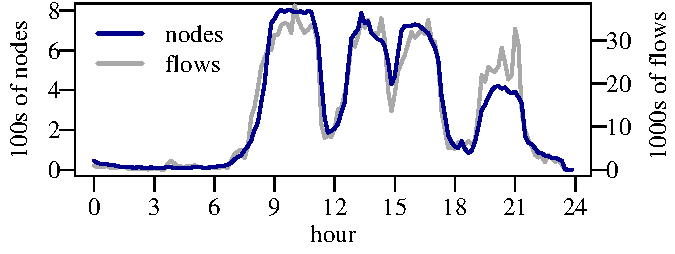
\includegraphics[width=3.3in]{nodes-flows}%
\vspace{-1.25em}%
\caption{The number of active nodes and flows over time.} 
\label{fig:nodes-flows}
\end{center}
\vspace{-1.3em}
\end{figure}


We do not assume or claim that the traffic found at \caps{IETF}60 is representative of conference settings in general. The observed behaviors are also unlikely to resemble those found in a typical commercial or residential setting. We have chosen this trace, however, because within it can be found behaviors resembling many different types of wireless usage cases. \Figure{nodes-flows} shows the wide variations in the number of active flows and nodes over the course of the trace. In the night and morning hours, the traffic patterns are similar to those one might find in a moderately trafficked business or residential area. During working group sessions, we see highly concentrated, heavy usage patterns. At the zenith of activity, over 800 users, 33 thousand flows, and 1 million packets are seen in a single 10-minute trace segment. At the nadir, a lone node sent only a single 61-byte packet over the course of 10 minutes. All levels of activity between these extremes are represented. Moreover, the mix of traffic types observed changes dramatically over the course of the day, providing a wide representation of possible blends of behavior. This heterogeneity and extreme range of behaviors makes the \caps{IETF} data set ideal for this evaluation. The variety of activity gives us greater confidence that success or failure of traffic models is not tied to any specific network condition, but is broadly and generally applicable. %For a traffic model to be truly realistic, it must be realistic across many different usage cases.

Before using the traces, it is necessary to extract application-level behavior from the trace header data. First, we split the trace into individual packet flows. A flow is a series of packets sharing the following five attributes: \caps{IP} and transport protocols (raw \caps{IP}, \caps{ICMP}, \caps{TCP}, \caps{UDP}); source and destination \caps{IP} addresses and \caps{TCP}/\caps{UDP} port numbers. Next, the quantity of application-initiated data contained in each packet is calculated. For non-\caps{TCP} packets, this quantity is simply the size of the transport-layer payload, but for \caps{TCP} the calculation is more complicated: only new data transfers, explicitly initiated by the application are counted. Data retransmitted by \caps{TCP} is disregarded, and empty \caps{ACK}s are ignored. \caps{SYN} and \caps{FIN} flags in packets (even empty ones) are counted as a single byte each, since they are explicitly signaled by the application. %After processing, we have a collection of flows, each with a sequence of timestamps and the amount of application-initiated data sent at that time.

\subsection{Simulations}
\label{sec:simulations}

We use the Qualnet wireless network simulator (version 4.0.1) to perform our experiments. We simulate a stationary multi-hop 802.11g network using the Ad hoc On-demand Distance Vector (\caps{AODV}) routing protocol~\cite{rfc:aodv}, with nodes placed randomly in a square field with sides of 150 meters.
In addition to the active nodes corresponding to trace \caps{IP}s, half as many passive ``infrastructure'' nodes are added to each simulation: these nodes initiate no data and simply serve as additional network relays. Our simulations resemble multi-hop mesh networks of the kind that are increasingly studied and deployed for delivery of broadband access in residential, corporate and conference settings. We do not attempt to reproduce the physical environment of the original wireless network, nor do we simulate mobility. The only aspect of the original network's behavior that is reproduced is the total pattern of network-wide traffic.

There are a number of potential objections to this approach. We use single-hop trace data to drive multi-hop simulations; the physical environment, node mobility, handover behavior, and closed-loop dynamics of the original wireless setting are not faithfully reproduced. One must keep in mind, however, that the goal of this research is \textit{not} to understand the conditions of the original network. Rather, we are using the traffic behaviors observed as examples to help us better understand how different types of workload can affect performance metrics. In particular, we aim to understand how real workload compares with common synthetic traffic models. Of course, the reason for such objections is that networking researchers understand that the many aspects of behavior interact with each other in a complex and nearly inextricable manner. However, before we can hope to understand the interaction between workload and other features affecting network behavior, we must study traffic patterns alone, and learn to model them with reasonable accuracy in the absence of additional complicating factors. Accordingly, in this study, we detach application level traffic patterns from the other factors influencing network conditions, and study them in isolation.

The 24-hour trace is split into 144 10-minute segments, each of which serves as the basis for a set of simulations using different traffic models. The traffic models range from a completely realistic trace-driven model, to a standard \caps{CBR} traffic model. Various partially synthetic intermediate models, described in \Section{traffic-models}, are simulated to study the impact of different aspects of traffic behavior on network performance. To preserve the fairness of the performance comparison, we keep as many features as possible constant across different traffic models. The traffic generated by each synthetic model preserves as many characteristics from the original trace as possible, within the constraints of the model. Moreover, the following features are preserved across all models: the number of wireless nodes, the number of flows, the number of application-initiated data units sent, the total bytes of application data sent, and the average flow duration (and therefore the average data rate).

In our previous work, we approximated \caps{TCP} with a pair of half-duplex \caps{UDP} flows~\cite{Karpinski07:realism,Karpinski07:cbr-failure}. For this work, we have implemented a new Qualnet application driver that allows trace-driven full-duplex \caps{TCP} flows. This allows us to accurately reproduce the full dynamics of \caps{TCP} feedback. Moreover, raw \caps{IP}, \caps{UDP} and \caps{TCP} flows are implemented using the same code, guaranteeing that all traffic is simulated uniformly and that all performance metrics are aggregated in the same manner. We have also instrumented Qualnet to collect \caps{IP} performance metrics in strict adherence to the recommendations of the \caps{IETF} working group on \caps{IP} performance metrics~\cite{rfc:ip-metrics}.

\subsection{Performance Metrics}
\label{sec:performance-metrics}

We have selected six performance metrics to present here. They are commonly used as indicators of network performance at the application, network, and link layers of the protocol stack:
\begin{enumerate}
\setlength{\itemsep}{0em}
\item \textbf{Application:} average end-to-end delay, packet delivery ratio, received throughput.
\item \textbf{Network:} \caps{AODV} control overhead (\caps{RREQ/RREP/\\RERR}), packets dropped in routing queues.
\item \textbf{Link:} 802.11 control overhead (\caps{RTS/CTS/ACK}).
\end{enumerate}
These metrics are commonly used to evaluate wireless protocols. We have examined a broad variety of other wireless network performance metrics, and although we do not have room to present or discuss them here, the results shown are representative of the overall realism of the traffic models.

\section{Results}
\label{sec:results}

%!TEX root = ../paper.tex

\begin{sidewaysfigure*}
\subfloat[\textbf{Application:} Average End-to-End Delay]
{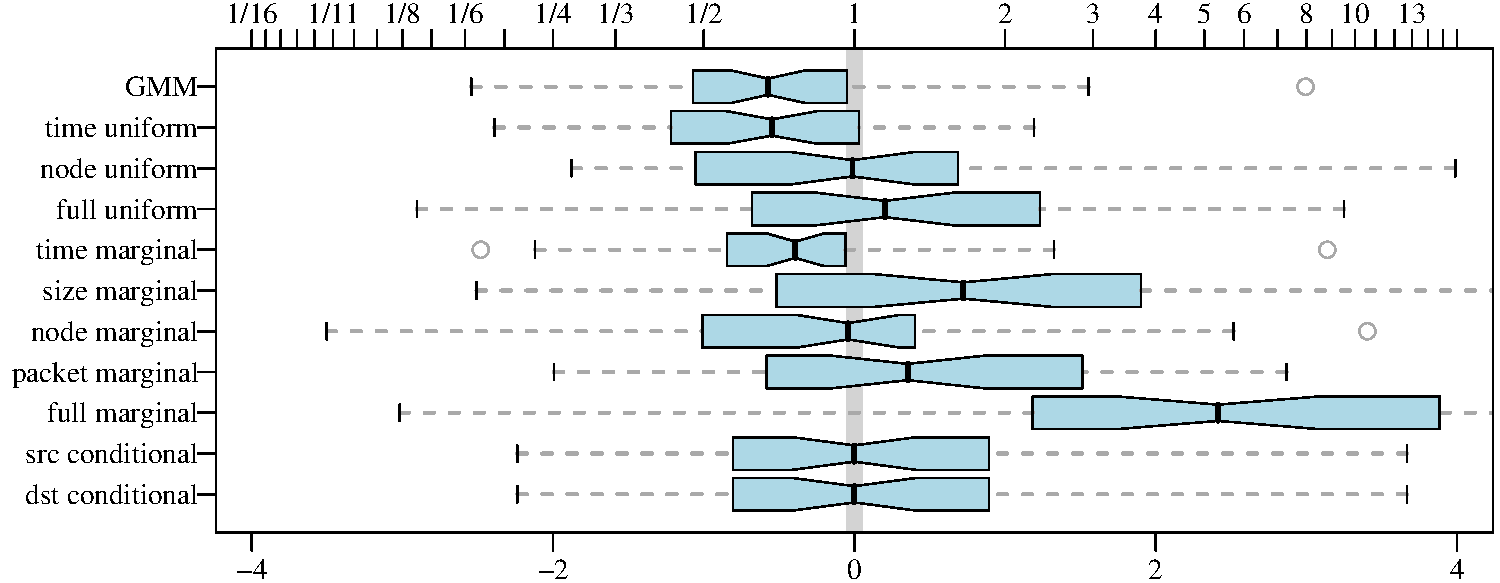
\includegraphics[width=4.6in]{Application/delay}}
\subfloat[\textbf{Application:} Packet Delivery Ratio]
{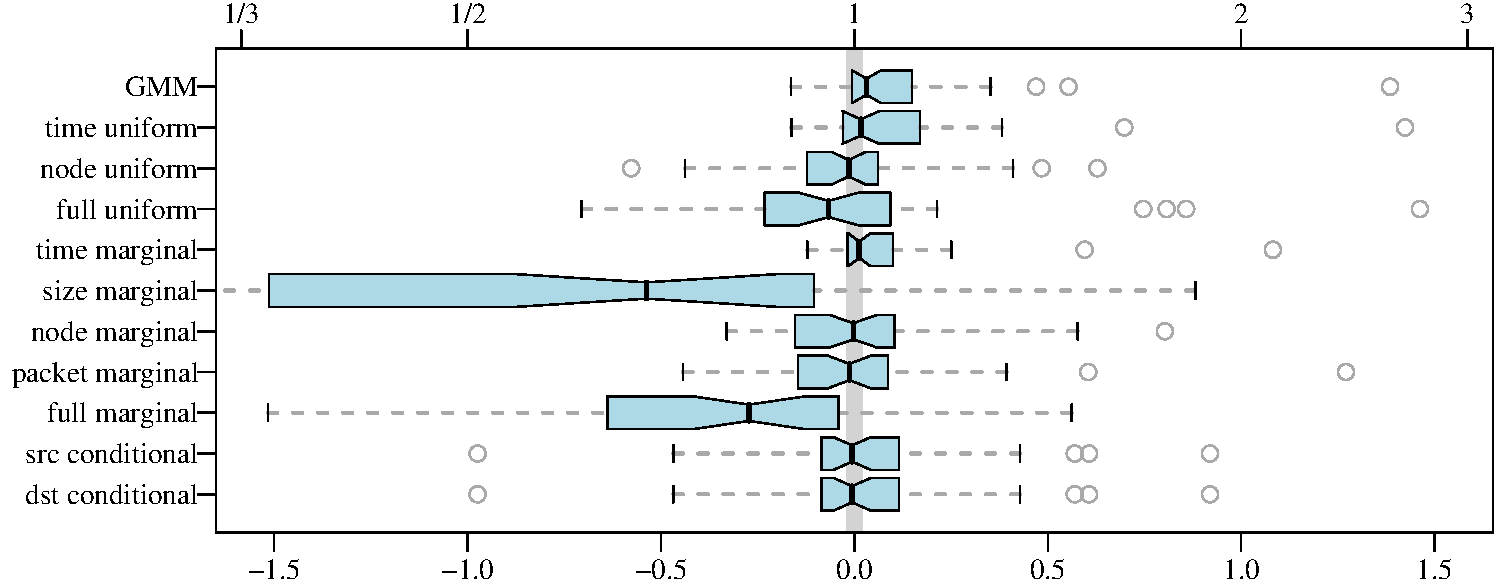
\includegraphics[width=4.6in]{Application/delivery_ratio}}

\subfloat[\textbf{Application:} Average Received Throughput]
{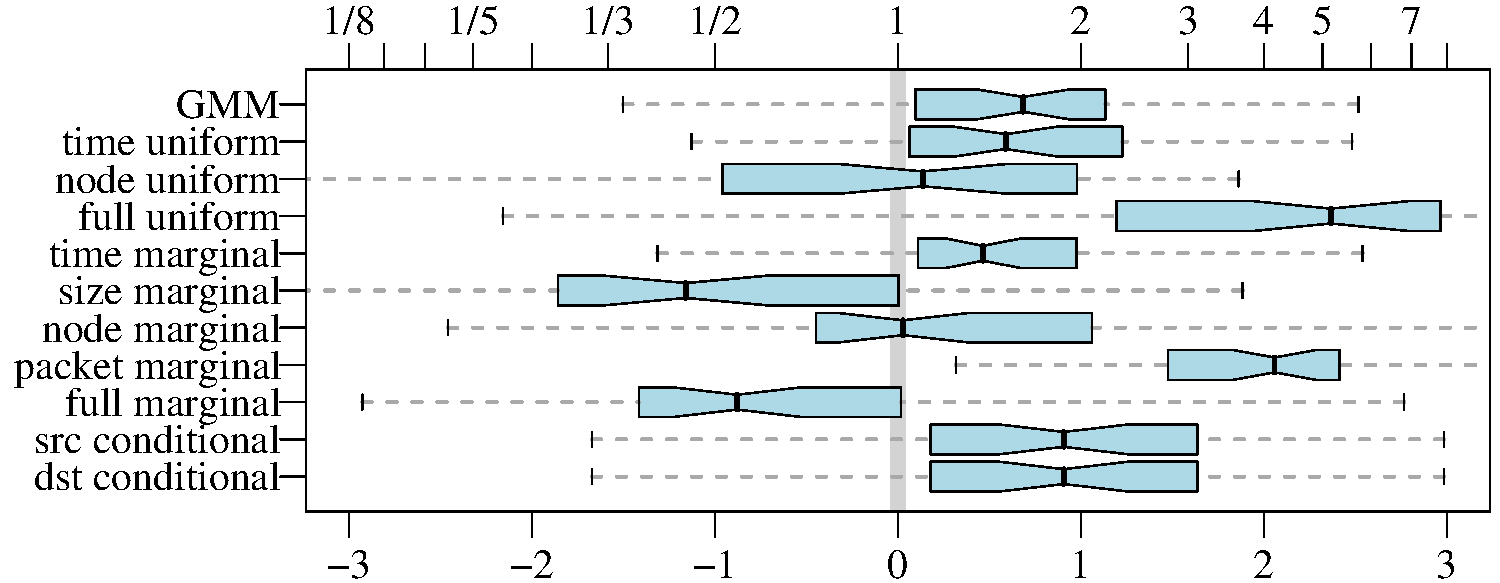
\includegraphics[width=4.6in]{Application/throughput}}
\subfloat[\textbf{Network:} AODV Control Overhead]
{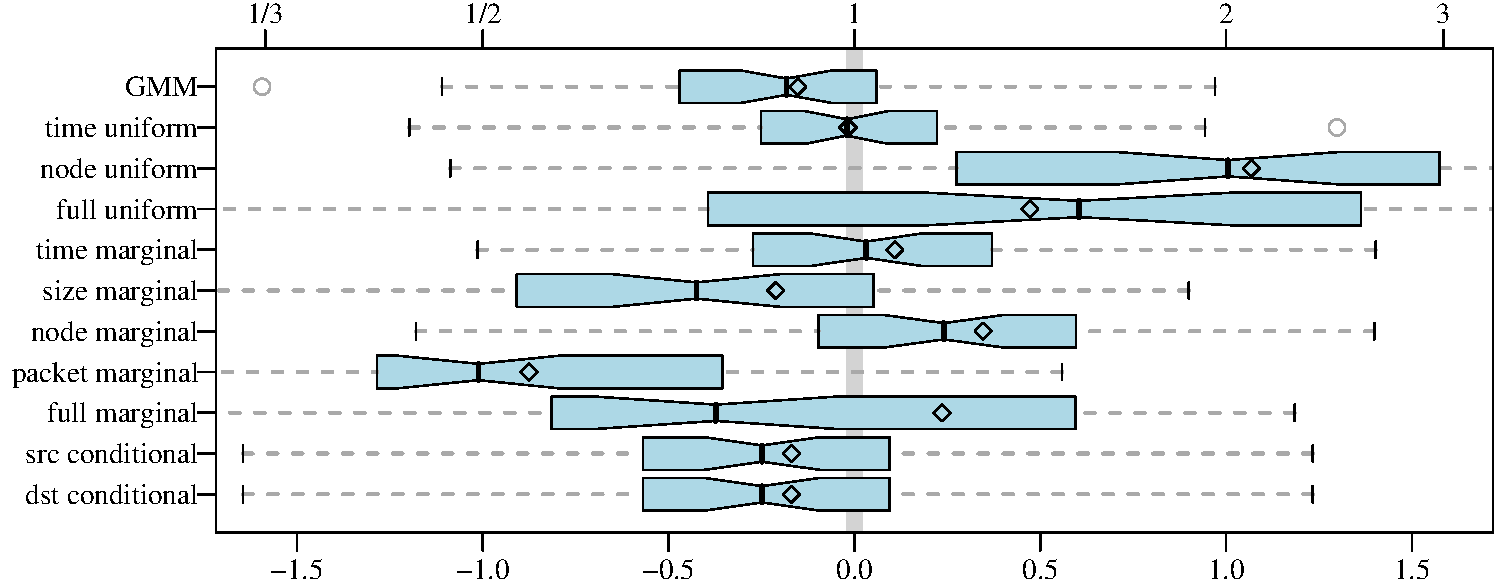
\includegraphics[width=4.6in]{Network/control_packets}}

\subfloat[\textbf{Network:} Packets Dropped in Routing Queue]
{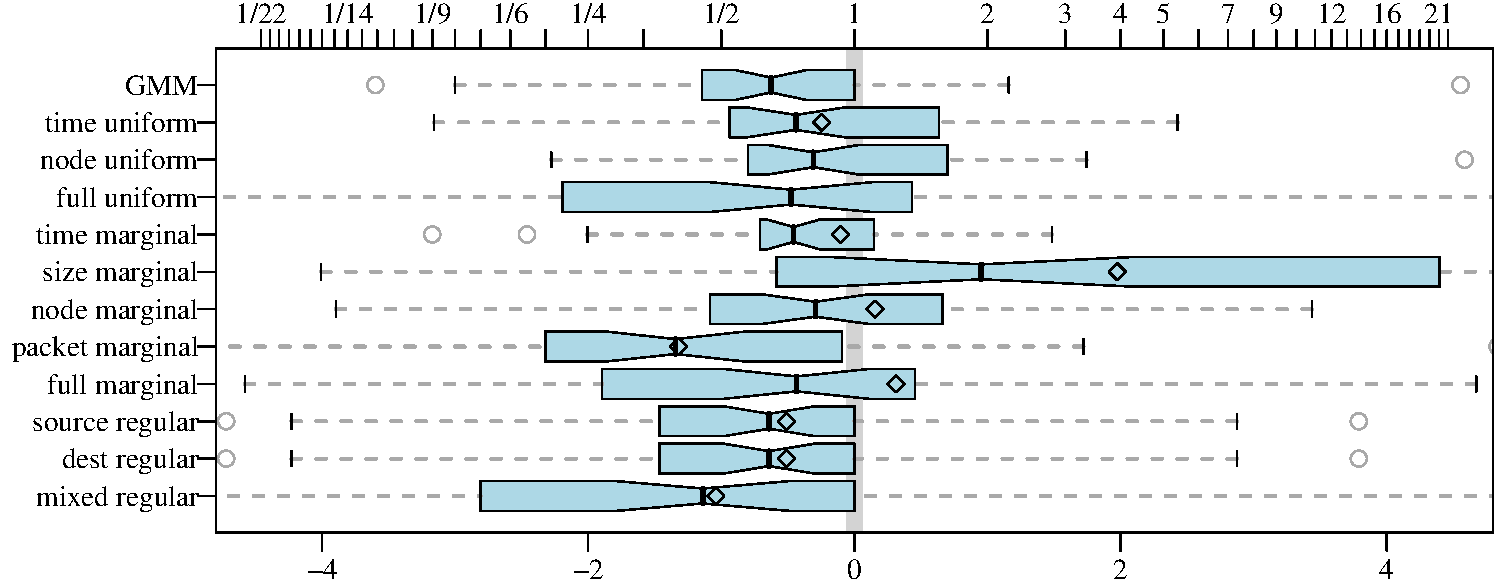
\includegraphics[width=4.6in]{Network/dropped}}
\subfloat[\textbf{Link:} 802.11 Control Overhead]
{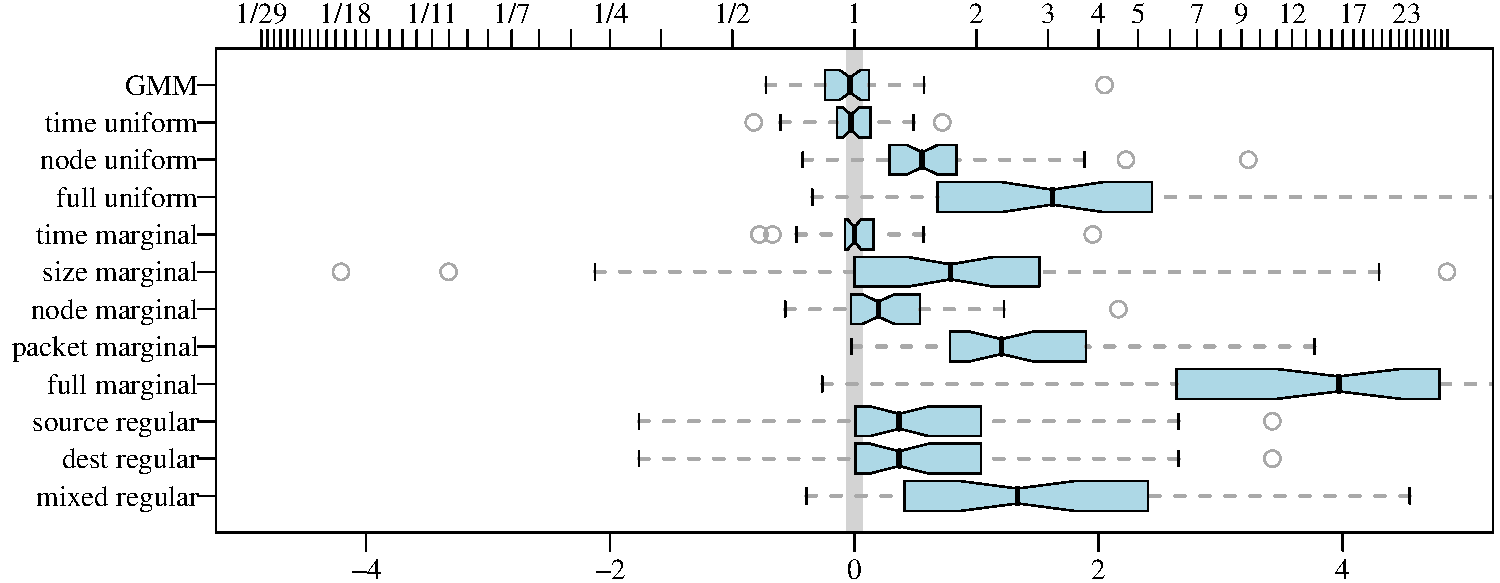
\includegraphics[width=4.6in]{Link/overhead}}
\caption{%
Box-and-whisker plots of log-ratio error values for all metrics and traffic models.
The lower axis indicates the log-ratio, while the upper axis shows raw ratio values.
Each box contains the central majority of log-ratio values:
the left and right bounds are at the $25^\text{th}$ and $75^\text{th}$ percentiles.
The dark middle line indicates the median value, while the diamond marks the mean.
The whiskers (dotted lines) extend to the furthest non-outlier values, while the points beyond that are outliers. The notch in the middle of each bar indicates a $95\%$ confidence interval for the true underlying median value;
if two notches do not overlap, they are very unlikely to have the same median.
}
\label{fig:box-plots}
\end{sidewaysfigure*}


Our simulation results are summarized in \Figure{box-plots}. Each subfigure shows a single performance metric. The distribution of log-ratio error values for each traffic model is visualized with a box-and-whisker plot. The box indicates the range from the 25th to 75th percentiles of values, while the ``whiskers'' indicate the full range, excluding outliners (which are shown as isolated points). These plots allow immediate assessment of realism: a good traffic model should have error values that are tightly clustered around the center, with a small, evenly balanced box, and relatively small whiskers. Additionally, the mean and median markers should be close to the center. It should be noted that the error scale is logarithmic, so even a slight increase in spread or deviation from the center indicates a disproportionately large decrease in model quality. Non-logarithmic scale markers are shown above each plot; the values indicate the factor of over- or under-representation for the performance metric.

The primary result is that the \caps{GMM} accurately reflects the performance of the trace data it is based on. It has small, centered error bars for every performance metric presented here, as well as for those we have looked at otherwise. This is an essential result, since otherwise, \caps{GMM} is at best a shaky foundation for further modeling work. With these results, we can be assured that if we can approximate the matrix for a given example of trace traffic, then we have also approximated the original trace behavior. In a sense, this result is a reduction of the general traffic modeling problem to a more tractable matrix modeling problem.

It is worth noting that \caps{GMM} has competition from a few of the time-simplified models: the \model{time marginal} and \model{time uniform} model both do approximately as well, and in some cases better, for the metrics examined. {\FHC} found strong evidence that session arrivals followed a time-varying Poisson arrival process, meaning that other than long-scale time-varying arrival rate and very small-scale clustering of flows within sessions, the overall flow arrival rate is fairly smooth. We suspect that on the scale of minutes to tens of minutes in which our simulation exist, it is sufficient to model both flow and session arrivals uniformly. This result indicates that the precise temporal placement of flows is not highly sensitive: they tend to be relatively evenly spaced out at short time-scales, and network performance is not sensitive to changes in start-time on that scale.

Not all marginal models have such a benign effect on the accuracy of performance metrics. The worst offender by far is the \model{size marginal} model. This model distorts behavior at every level, by more than a factor 20 in 25\% of scenarios in the case of routing queue packet drops. This is a highly significant result because modeling flow size using a network-wide marginal distribution is precisely what {\FHC}, for example, attempt. This results informs us that this approach is doomed to failure: flow size cannot be assigned without considering its relation to other flow properties: source and destination nodes, and packet behavior at the very least.

The \model{packet marginal} model is another offender, albeit not as egregiously. The direction of the misrepresentations in this case, however, is more dangerous: received throughput is overestimated by more than three times, 75\% of the time. On the other hand, \caps{AODV} control overhead is underestimated by half on average. Such serious misrepresentations are especially noteworthy given the apparently innocuous assumption applied by this model: the \model{packet marginal} model is essentially a standard variable bit-rate (\caps{VBR}) packet behavior model, using the empirical network-wide distributions of packet sizes and inter-packet intervals. Otherwise the model matches the original trace behavior exactly. And yet these drastic distortions occur. In our previous work, we have shown similarly drastic misrepresentations to occur when constant bit-rate packet behavior is assumed. This results indicates that to reproduce accurate network performance, we must provide packet behaviors on a more granular level: each node or even each flow must be assigned a ``custom'' packet behavior by some means.

These strong negative results for two fundamental and very common marginal models provide severe limits on the realism that can be achieved through marginal modeling. Traffic modeling research \textit{must} move beyond simply finding parametric models for marginal distributions of network-wide properties. Realistic behavior cannot be generated using these distributions alone. Something must be captured about the interaction between the elements of flow behavior.

Finally, we turn to the conditional models. These demonstrate neither exceptionally good nor exceptionally bad behavior. That the conditional models should be similar to the \model{full marginal} model but somewhat more realistic is entirely expected: conditioning, the reader will recall, is a restricted form of marginal modeling, where each group of flows has its own marginal distribution. In these cases, the flows are grouped by source node or by destination node.

% The mixed case uses the average behavior of the other two cases. It is interesting to note that the mixed case is universally worse than either the source or destination case. Clearly, hybridizing the conditioning here is not an effective technique. We believe that the cause of this effect is like mixing too many colors yielding an unpleasant shade of brown: any of the colors individually would be better than the nondescript average. As a more general conclusion, arbitrarily mixing model may not always be a good idea, despite the ease with which it is done in the matrix representation of workload behavior.

%We also believe that the fact that both the \model{time marginal} and \model{time uniform} models perform about as well as the \caps{GMM} indicates not that they are performing exceptionally well, but that the \caps{GMM} is performing worse than it should in this case. This may be an artifact of the interaction between packet behavior, flow size, flow duration and start time, as described in \Section{traffic-generation}. This remark may appear to be a non-sequitur, but these properties are all closely related. Consider that packet behavior (i.e. distribution of packet sizes and inter-packet intervals) determines the expected mean packet size and expected mean interval duration. The expected duration is then related to the flow size via the following equation:
%\begin{align*}
%\E{\text{duration}} = [\text{flow size}]\frac{\E{\text{mean interval}}}{\E{\text{mean size}}}
%\end{align*}
%The duration must also satisfy $t_{\text{start}}+[\text{duration}] \le t_{\max}$.

%It accurately reproduces important performance metrics at all levels of the protocol stack in simulation. This only moves us a step closer to being able to generate realistic, completely synthetic workloads, since the \caps{GMM} in these comparisons  derives almost all of its behavior directly from the trace. However, it means that we have effectively reduced the problem of generating realistic workload to the problem of classifying and understanding what sorts of traffic matrices occur in real workloads. Moreover, we can express a vast array of different approaches to traffic modeling simply and uniformly using matrix operations.

\section{Discussion}
\label{sec:discussion}

%The story of network analysis and modeling is one of variety. Assumptions of ``sameness'' have fallen repeatedly. ...
%The matrix model gives new insight into 

Thus far, we have addressed two out of three of the originally posed questions regarding traffic modeling. First, we have proposed a general approach for representing whole-network traffic without making assumptions of uniformity or marginality. To this end, we introduced the concept of a linear representation of traffic. The general matrix model entails a specific linear representation, such that network traffic patterns can easily be expressed as matrices. Our experimental results show that the \caps{GMM} is sufficiently realistic for generating wireless workload derived from traces. When uniform or marginal assumptions are applied, however, sufficient realism eludes us, indicating that if we are to simplify and reduce the representation of network behaviors, we must do some through some other technique. In \Section{modeling-concepts}, we observed that application of uniformity and marginality assumptions to traffic instances is equivalent, in the \caps{GMM}, to right and left multiplication, respectively, by matrices of rank one. These transformations destroy almost all of the information in the original traffic matrix---only the zero matrix has lower rank than these.

The question that remains to be answered is how we can simplify and reduce the representation of network behaviors without making unwarranted and intuitively clearly false assumptions of uniformity of marginality of network behaviors. We present here preliminary results from applying non-negative matrix factorization to the packet behaviors of collections of flows. Recall from \Section{general-matrix-model}, that the matrices $Z$ and $V$ represent the packet size and inter-packet interval histograms of a collection of flows, with each row corresponding to a flow, and each column corresponding to a packet size or a range of inter-packet intervals. We apply \caps{NMF} to the concatenation of these matrices, $\mat{P}=[\mat{Z}~\mat{V}]$. \caps{NMF} attempts to approximate $\mat{P}$ as the product of three non-negative matrices:
\begin{align}
\mat{P} \approx \mat{W}\mat{\Sigma}\mat{H},
\end{align}
where $\mat{W} \in \R^{f \times K}$ is row-stochastic,
$\mat{\Sigma} \in \R^{K \times K}$ is diagonal with descending diagonal entries, and
$\mat{H} \in \R^{K \times (d_z+d_v)}$ is row-stochastic as well.
$K\in\N$ is the rank of this factorization, which must be determined somehow as well.
What is the interpretation of such factorization?
The rows of $\mat{H}$ are \emph{basic behaviors}---pairs of packet size and inter-packet interval distributions, such that each flow's packet behavior can be approximated as a linear combination of these basic behaviors.
Specifically, the matrix $\mat{M}\mat{\Sigma}$ gives the mixing coefficients for each flow.
The diagonal entries of $\mat{\Sigma}$ have a special meaning as well:
they are the number of packets associated with each basic behavior.
Thus the basic behaviors are sorted in descending order of how much traffic they explain.
Note that the factorization does not associate basic behaviors with individual packets;
rather, total flow behavior is explained as a mixture of basic behaviors, so the fraction of packets in each flow explained by a given behavior is known, while the specific packets are unknown.

The striking results of applying non-negative matrix factorization to $\mat{P}$ are shown in \Figure{basic-behaviors}. Twelve basic behaviors suffice to explain all the traffic in a ``toy''  sample of 4138 flows. The pairs of packet size and inter-packet interval distributions are almost immediately recognizable as resembling intuitive modes of network behavior. The first basic behavior, for example has all packets near the \caps{MTU}, while intervals are smoothly distributed around a fraction of a millisecond. This is what we would expect from downloading large files; and indeed, the breakdown of packets by port number bears out this interpretation---almost all of the traffic is \caps{HTTP} server traffic, with small slivers of \caps{IMAP} and \caps{SSH} server traffic. The second basic behavior is equally intuitive: tiny packets with frequency distributed around 0.1 seconds---this is all \caps{SSH} traffic, interacting with a remote terminal via keystrokes and screen updates.

%!TEX root = ../paper.tex

\begin{sidewaysfigure*}
{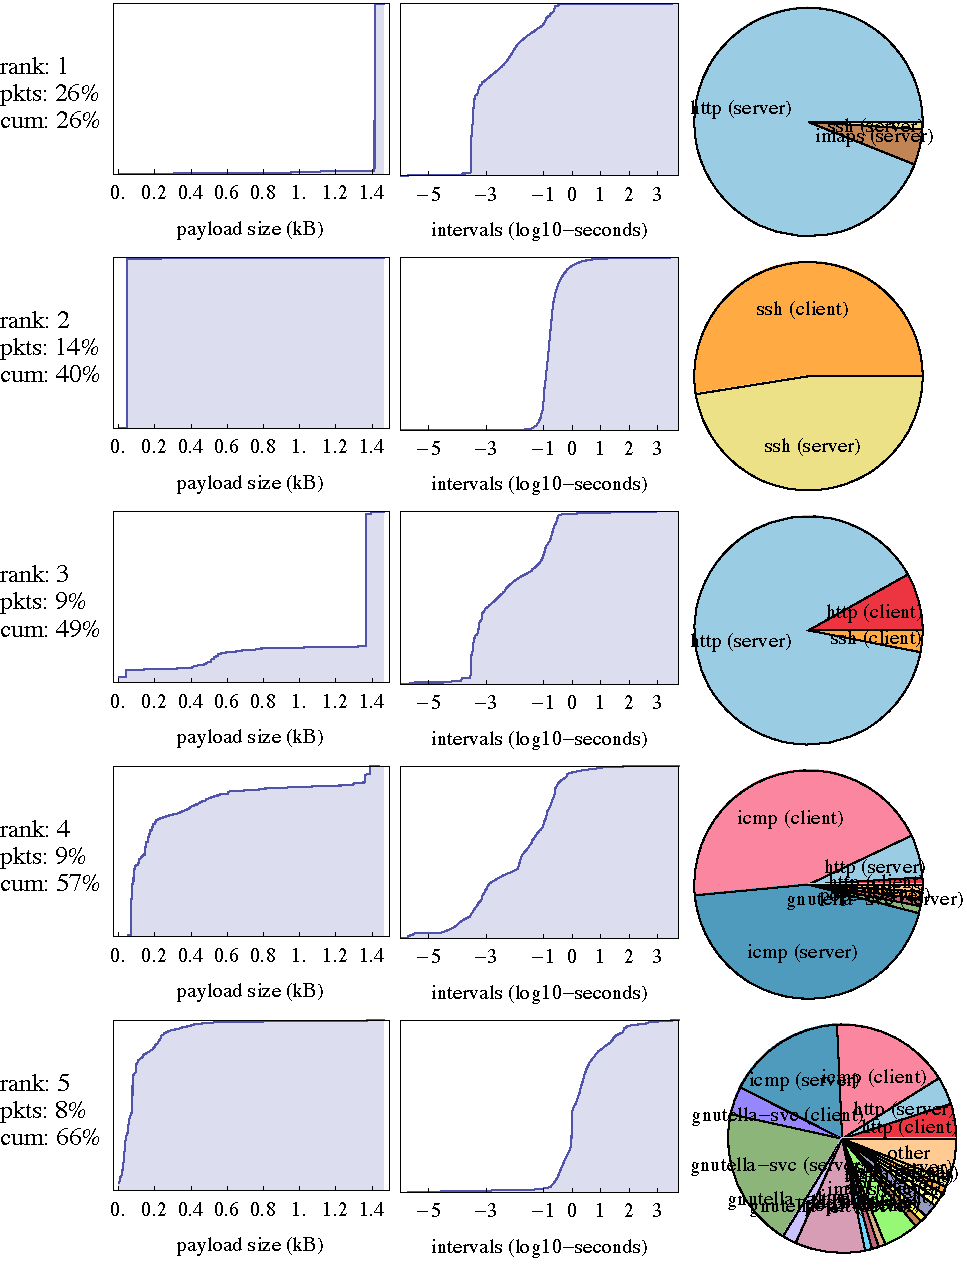
\includegraphics[height=5.95in]{basic_behaviors_1.pdf}}\hfill%
{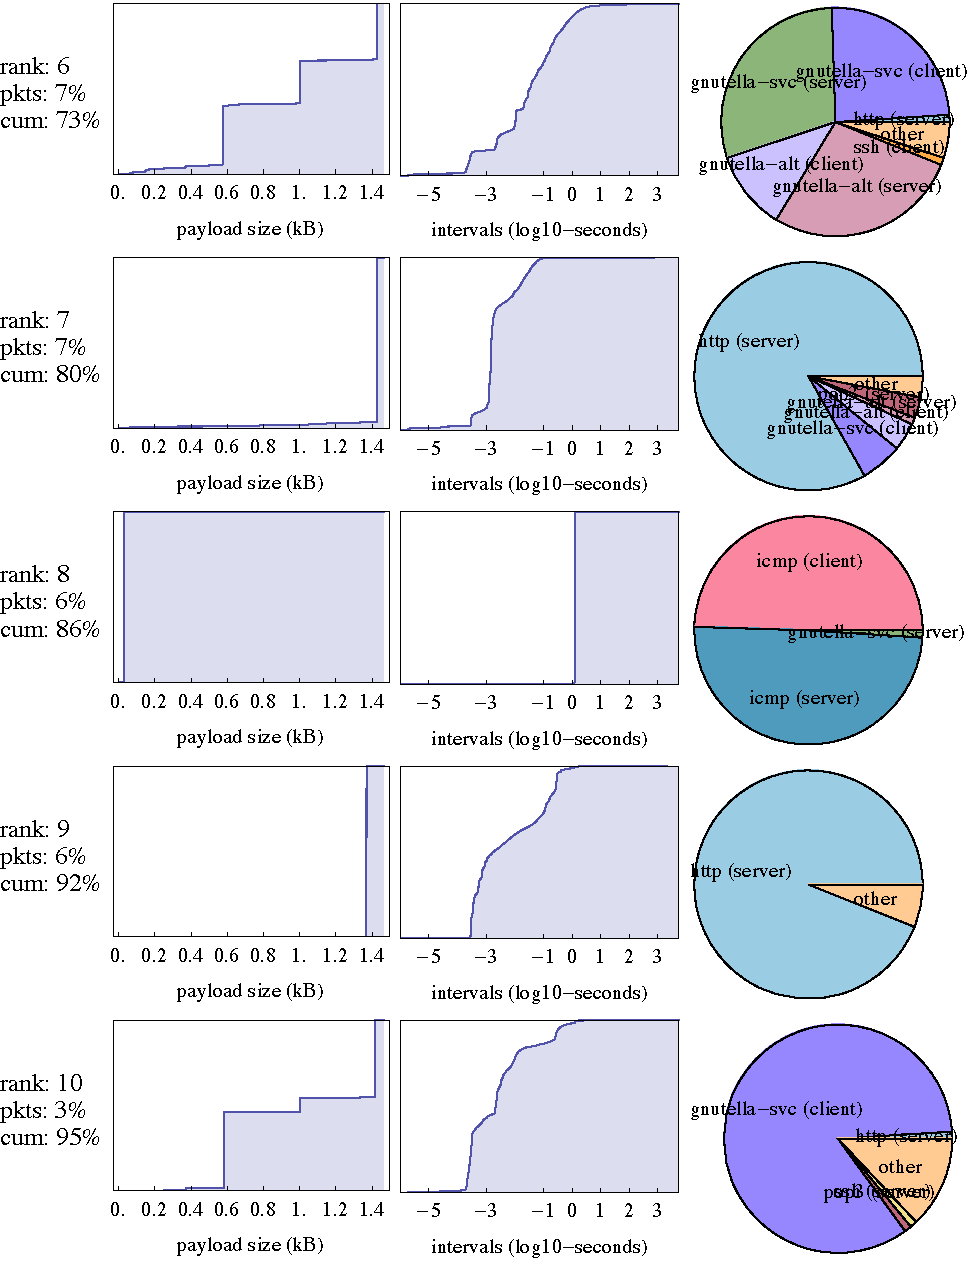
\includegraphics[height=5.95in]{basic_behaviors_2.pdf}}
\caption{%
The ten most prevalent components of flow behavior as pairs of packet payload size and of inter-packet interval distributions.
The distributions are shown as cumulative distribution functions: the $x$-axis represents payload size (in kilobytes) or inter-packet interval duration (in log-seconds, base 10), respectively;
the $y$-axis indicates the probability a value occurring, less than or equal to the $x$ value.
The behaviors are ordered in descending rank of how many packets they explain;
to the left, each behavior's rank is indicated, together with the percentage of total packets associated with it, and the cumulative percentage of packets explained.
To the right of each behavior is a pie chart showing the breakdown of associated packets by protocol, as determined by well-known port numbers.
}
\label{fig:basic-behaviors}
\end{sidewaysfigure*}


% What are the ramifications of these results? In our previous work, we had already demonstrated the drastic distortions that are introduced by uniformity assumptions made by the most common traffic models. This work serves to further critique established common assumptions in traffic modeling. The strongest message to be taken away is that the aspects of traffic behavior of both nodes and flows \textit{must} be considered jointly. It is not sufficient to continue modeling marginal distributions of network properties. These marginal models do not lend them selves easily to traffic generation in the first place, and when marginality assumptions are applied to trace traffic, the result is a severe distortion of important network performance characteristics. It is now well established that network traffic patterns have an impact on network performance that cannot be ignored. Even experimental deployments cannot avoid the need for more realistic traffic workload models. While using a real, physical network successfully sidesteps simulation problems below the application layer, without realistic traffic models, reliable, meaningful performance predictions remain beyond our reach.

%\subsection{Generality of Results}

%% TODO: talk about other synthetic models not considered here.
%% The point of our analysis is not to show that no synthetic models can be accurate, but rather, that the commonly used models, and obvious variations thereof, are not accurate.

%The most significant limitation on the generality of this analysis is that it is based entirely on a single data set from \caps{IETF}60---albeit a large and varied one. It is possible that traffic in this trace happens to produce network performance that is unusually dissimilar to standard traffic models. This data set, however, represents a highly heterogeneous collection of network usage behaviors, from slow and steady off-peak usage, to extremely heavy peak usage: over 800 users, 33 thousand flows, and 1 million packets in a single 10-minute trace segment. Despite the broad variety of behaviors, the results are consistent: in all types of usage scenarios, simplistic traffic models, like uniform \caps{CBR}, systematically skew important performance measurements at all levels of the network. While the precise results for other data sets might differ, it is very unlikely that \caps{CBR} traffic models will happen to accurately reproduce realistic performance in other experiments. This paper provides strong evidence that better traffic models are needed for performance evaluations.

% \subsection{Towards Realistic Models of Wireless Workload}
% 
% What would better traffic models look like? How can we create them? One possible approach is to use actual traffic traces as we have done. This approach is unsatisfactory, however, because it provides the experimenter with almost no control over experiments. Synthetic models have parameters, which can be tweaked as necessary---adjusting, for example, the number of active nodes in a simulation, without affecting other parameters. Traffic traces, on the other hand, must be used without significant alteration if they are to actually provide the desired realism. This inability to control all but one or two parameters is nearly crippling for experimental purposes. Therefore, the research community needs models whose parameters can be adjusted independently, but whose performance characteristics can be made to resemble whatever example of network behavior one might need. The general matrix model does not yet fulfill this role since its parameters cannot be freely varied. We believe, however, that \caps{GMM} plays a vital role in the ongoing process of developing  of better models. By reducing the general problem of traffic modeling to the domain of linear algebra, we have provided traffic researchers with a vast array of powerful theoretical and computational tools that can be immediately applied to the problem at hand.\footnote{The derived models used in this paper were all implemented in Matlab, each in only a few simple lines. All the models used here are implemented in only 19 total lines of code. Of course, the framework to apply them to traffic traces and simulations is somewhat larger.} What are the next steps? The authors are currently investigating a variety of matrix factorization and clustering techniques to extract hidden structure from a large and diverse body of real traffic.

%The reader will note that the transformations applied in this paper are all quite simple. Our conditioning matrices primarily consisted of ones and zeros. The algebraic representation of complete workload 

%The ``messiness'' of the performance comparison from trace data in Figure~\ref{fig:mac-control-overhead-cmp} illustrates why using traces directly is not ideal: each data point differs not only in the number of nodes shown on the $x$-axis, but also in other dimensions, such as the number of flows and packets, and the average flow duration. The result is a highly noisy comparison, affected by many unseen parameters. Only by applying a local smoothing algorithm are trends somewhat elucidated.

%Instead of using trace data directly, it should be possible to configure a synthetic traffic model based on observations from a real data set, and then run side-by-side simulations using the synthetic model and the real data, producing statistically equivalent performance results. This is precisely what our definition of sufficient realism entails. The work in this paper provides the tools to measure how close to this ideal a model is and in what areas it needs improvement. Without this feedback, any improvements in realism are purely guesswork. Our breakdown of traffic behavior into three orthogonal levels also allows the problem to be approached in smaller pieces, rather than being solved all at once.

%The next step towards better traffic models is to investigate which aspects of real traces may be altered without detrimentally affecting the resulting performance metrics. For example, to test whether a complex time-series model of packet behavior is necessary, we randomize the order of the packet sizes and/or inter-packet intervals and compare performance using these randomized traces against performance using the original traces. If the performance is unchanged, we can conclude that no complex time-series model of packet behavior is necessary: sampling the packet sizes and inter-packet intervals from empirical distributions is sufficiently realistic. If, on the other hand, the performance characteristics are altered by shuffling packets, then some time-series model of packet behavior is needed. By partially randomizing the packet order in specific ways, the exact limits of realism necessary can be found. A similar approach will allow the development of realistic models for the other levels of network usage behavior.

\section{Conclusions}\label{sec:conclusions}

%The real significance of this paper lies not in showing that the commonly used \caps{CBR} traffic model is unrealistic. Networking researchers understand that \caps{CBR} is at best a na\"ive approximation of real network traffic. Nor is the real significance that we have quantized the high degree of inaccuracy that can be induced by using this model. The real significance of this paper lies in providing an well-defined, objective measure of realism for traffic models. This has never previously existed: evaluations of realism have relied on essentially arbitrary statistical measures of similarity to real traffic. Existing traffic generators use empirical distributions of such quantities as file size, inter-connection time, packet size, or inter-packet intervals. They can only hope that reproducing these distributions as good enough. Without an external measure of accuracy, there's simply no way to know.

%attempting to showing that existing models are unrealistic, or that new models are more realistic have always focused on arbitrary statistical measures. A 

We have presented a fundamentally new, algebraic way of representing traffic patterns in local area networks. We call this representation the general matrix model. Each flow of a traffic collection is represented as a single high-dimensional vector with components representing the \caps{IP} protocol type, source and destination nodes, start time, flow size, and packet behavior. The essential property of the algebraic representation is that standard vector operations compute natural and useful descriptions of aggregate behavior over the collection of flows represented. Our experimental validation demonstrates clearly that the general matrix model accurately reproduces the performance characteristics of of real traffic. The benefits of a performance-preserving algebraic representation are multifold. The algebraic forms of the simplifying assumptions made by many common modeling approaches provide unprecedented clarity and coherence to a complex and confusing subject. For example, assumptions that various aspects of flow behavior are stochastically or deterministically uniform all take the same form algebraically: left matrix multiplication. The other major class of common simplifying assumptions made by traffic models is to apply some marginal behavior across the entire collection of flows or to disjoint subsets of the flows. Such simplifications correspond to right matrix multiplication in \caps{GMM}. Because of the simplicity and clarity that the algebraic structure brings to the subject, we can see clearly now that both common types of simplifying assumptions are na\"ive and simplistic. Our experimental results bolster this conclusion: both uniform and marginal models significantly misrepresent many important network performance metrics. With the general matrix model, however, we stand poised to use the powerful tools of modern linear algebra to develop general, elegant and powerful models of network behavior that just work.

%This research rigorously quantifies the impact of a variety of synthetic traffic models on performance metrics that wireless researchers use to evaluate new technologies and protocols. The first step in this assessment process was to formally define what it means for a network usage model to be sufficiently realistic. In essence, a model is considered realistic if it produces performance results that are statistically equivalent to those produced by real usage.
%A well-defined, objective measure of realism for traffic models has not previously existed. Evaluations of realism have formerly relied on essentially arbitrary statistical measures of similarity to real traffic, which may or may not affect the performance metrics that researchers care about.
%The definition of sufficient realism leads us to our general experimental approach: we use differential analysis comparing performance metrics derived from real traffic with those derived from synthetic traffic models. The theoretical contributions of this analysis are:
%\begin{enumerate}
%\item An in-depth analysis of the desirable mathematical properties of a measure of error for performance metrics.
%\item Proof that the unique measure of error that satisfies these properties is the log-ratio of metric values.
%\item Three rigorous tests of statistical equivalence between synthetic and real performance results.
%\end{enumerate}
%These analytical tools allow the evaluation of realism over a collection of drastically different usage scenarios. Evaluation over a heterogeneous collection of scenarios is essential to establishing the credibility of usage models. Moreover, these theoretical results are equally applicable to other types of usage models---for example, mobility.

%On the practical side, this paper gives crucial insight into why most researchers do not trust simulation results: with the traffic models commonly used, the results are unlikely to reflect real performance. Moreover, this problem will also hamper experiments in test-bed wireless networks, so long as the same na\"ive workload models are used. The only way to address this fundamental lack of realism is to develop usage models that reproduce important performance metrics more accurately. Our theoretical results provide the tools necessary to do this. The development of better traffic models should begin with real traces, and proceed by incremental changes, checked by differential analysis.
%%First, alter a small aspect of the trace, simulate, then compare. If the realism of the results is unaffected, the traffic feature altered was inessential. Otherwise, it is a feature of behavior that must be captured in a realistic traffic model.
%This approach will allow the precise mapping of which aspects of traffic patterns have an impact on performance and which ones can be safely abstracted away.
%% TODO: maybe cut out some of this last bit.

%\section{Acknowledgments}
%This work was funded in part through NSF Career Award CNS-0347886.

% Hernandez06:dissertation: ``complete methodology for reproducing the traffic observed on a network link in a closed-loop manner, and proposed a number of metrics for studying the realism of the generated traffic.''
\bibliographystyle{plain}
\bibliography{references}

\end{document}

